\documentclass[a4paper, 12pt]{article}
\usepackage[utf8x]{inputenc}
\usepackage[english, russian]{babel}
\usepackage[left=25mm, top=25mm, right=25mm, bottom=25mm]{geometry}
\usepackage{cmap}
\usepackage{indentfirst}
\usepackage{tikz}
\usepackage{float}
\usepackage{amsmath, amsfonts, amssymb}
\usepackage{graphicx}
\usepackage{hyperref}
\usepackage{listings}
\usepackage{caption}
\usepackage{subcaption}
\usepackage{xcolor}
\usepackage{etoolbox}
\usepackage{titlesec}
\usepackage{array}
\pagestyle{plain}
\patchcmd{\tableofcontents}{\contentsname}{\centering\contentsname}{}{}
\titleformat{\section}[block]{\normalfont\large\bfseries\centering}{}{0pt}{}
\titleformat{\subsection}[block]{\normalfont\normalsize\bfseries\centering}{}{0pt}{}
\allowdisplaybreaks
\graphicspath{{src/images/}}
\usetikzlibrary{patterns}
\definecolor{LightGray}{gray}{0.95}
\definecolor{LightGray2}{gray}{0.7}
\hypersetup{
    colorlinks=true,
    linkcolor=blue,
    filecolor=magenta,
    urlcolor=cyan,
    pdftitle={contents setup},
    pdfpagemode=FullScreen,
}


\begin{document}
    \begin{titlepage}

        \begin{center}
        Федеральное государственное автономное образовательное учреждение высшего образования
        «Национальный Исследовательский Университет ИТМО»
        \vfill
        
        
\includegraphics[width=0.3\textwidth]{itmo.png} % requires /src/images/itmo.png

        {\large\bf ЛАБОРАТОРНАЯ РАБОТА №1}\\
        {\large\bf ПРЕДМЕТ «ЭЛЕКТРОННЫЕ УСТРОЙСТВА СИСТЕМ УПРАВЛЕНИЯ»}\\
        {\large\bf ТЕМА «ИССЛЕДОВАНИЕ РЕГУЛИРУЕМЫХ СХЕМ НА ТИРИСТОРАХ»}\\
        Вариант №1
        \vfill

        \begin{flushright}
            \begin{minipage}{.45\textwidth}
            {
                \hbox{Преподаватель:}
                \hbox{Жданов В. А.}
                \hbox{}
                \hbox{Выполнил:}
                \hbox{Румянцев А. А.}
                \hbox{}
                \hbox{Факультет: СУиР}
                \hbox{Группа: R3341}
                \hbox{Поток: ЭлУСУ R22 бак 1.2}
            }
            \end{minipage}
        \end{flushright}
        \vfill
  
        Санкт-Петербург\\
        2025
        \end{center}
    \end{titlepage}
    
    \tableofcontents

    \newpage
    \section{Задание 1}
    \begin{figure}[H]
        \centering
        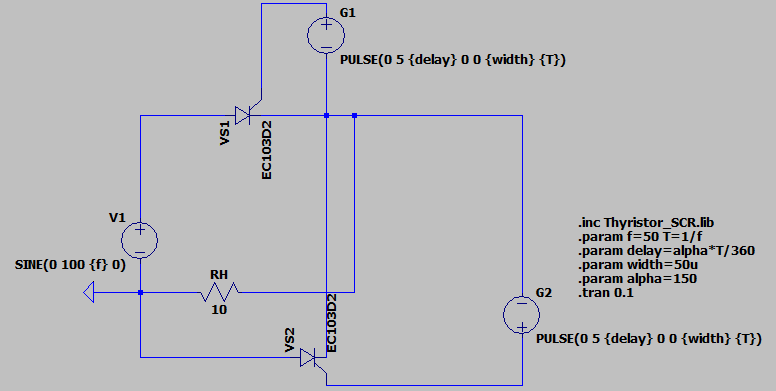
\includegraphics[scale=0.22]{scheme1.png}
        \captionsetup{skip=0pt}
        \caption{Подпись к изображению}
        \label{fig:scheme1}
    \end{figure}


    \subsection{Вых}
    \begin{center}
    \begin{tabular}{ | m{5em} | m{1.5cm}| m{1.5cm} | m{1.5cm} | m{1.5cm} | m{1.5cm} | } 
    \hline
    Угол $\alpha,\left(^\circ\right)$& 30 & 60 & 90 &120 &150 \\ 
    \hline
    $U_{\text{вых}}$, В& 55.1380 & 44.3180 & 29.4850 &14.6660 &3.8619\\ 
    \hline
    \end{tabular}
    \end{center}


    \begin{figure}[H]
        \centering
        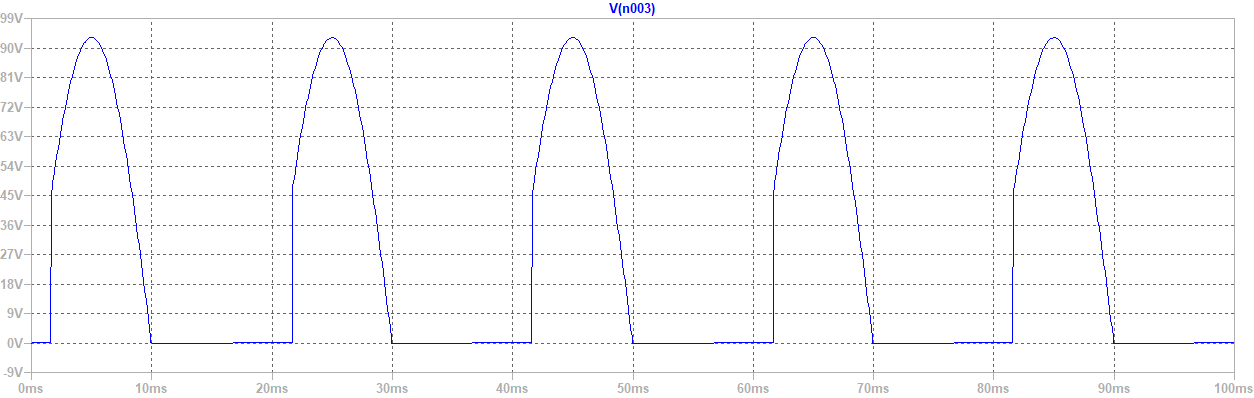
\includegraphics[scale=0.45]{a30.png}
        \captionsetup{skip=0pt}
        \caption{Подпись к изображению}
        \label{fig:a30}
    \end{figure}
    \begin{figure}[H]
        \centering
        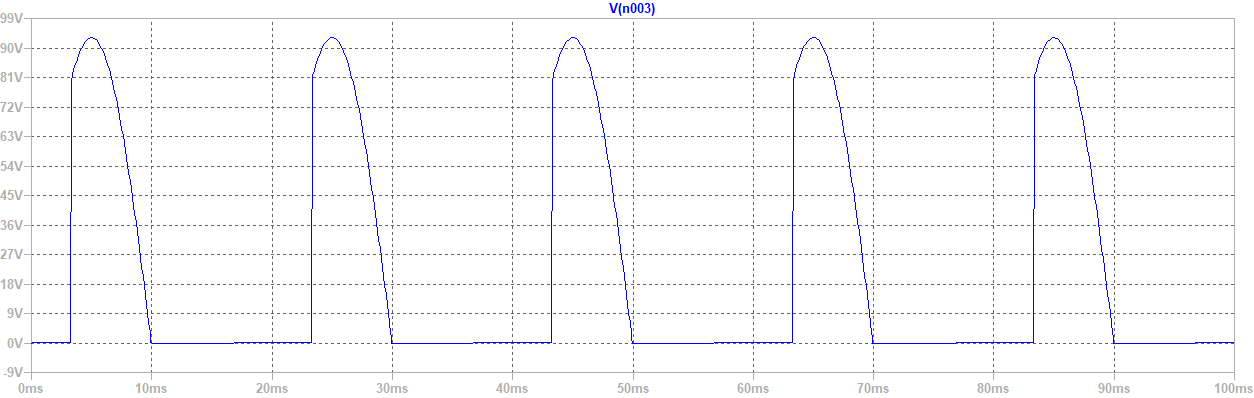
\includegraphics[scale=0.45]{a60.png}
        \captionsetup{skip=0pt}
        \caption{Подпись к изображению}
        \label{fig:a60}
    \end{figure}
    \begin{figure}[H]
        \centering
        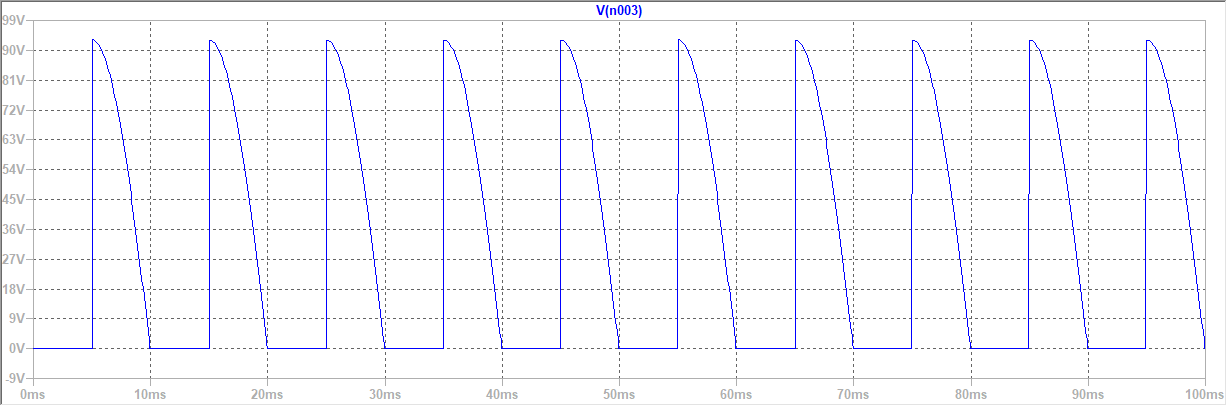
\includegraphics[scale=0.45]{a90.png}
        \captionsetup{skip=0pt}
        \caption{Подпись к изображению}
        \label{fig:a90}
    \end{figure}
    \begin{figure}[H]
        \centering
        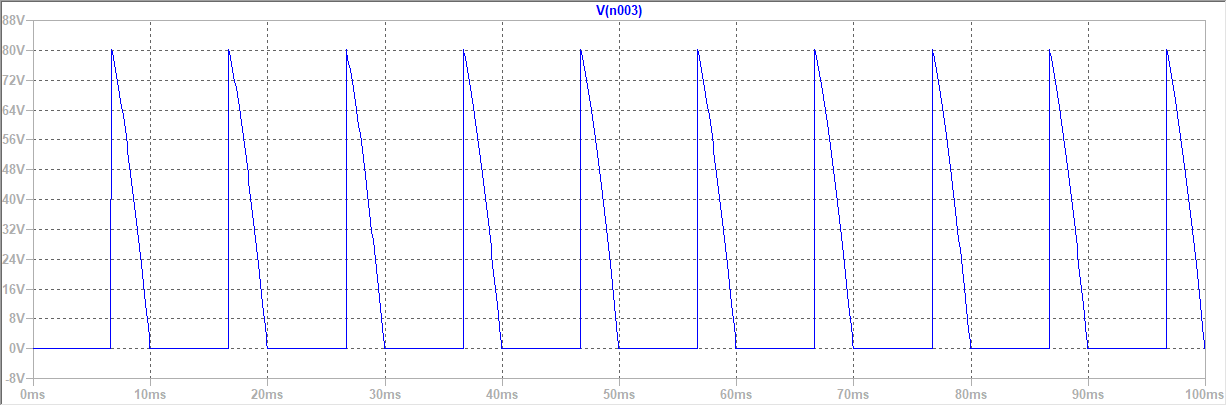
\includegraphics[scale=0.45]{a120.png}
        \captionsetup{skip=0pt}
        \caption{Подпись к изображению}
        \label{fig:a120}
    \end{figure}
    \begin{figure}[H]
        \centering
        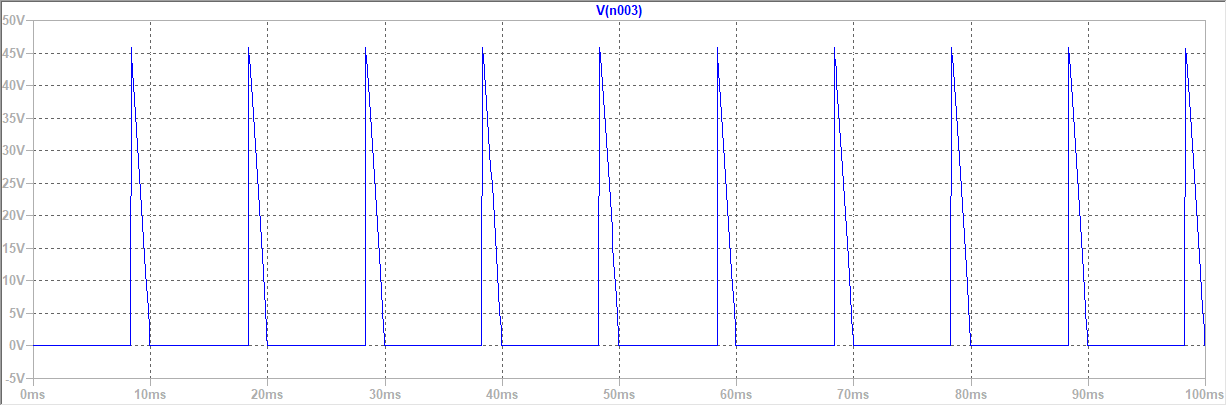
\includegraphics[scale=0.45]{a150.png}
        \captionsetup{skip=0pt}
        \caption{Подпись к изображению}
        \label{fig:a150}
    \end{figure}


    \begin{figure}[H]
        \centering
        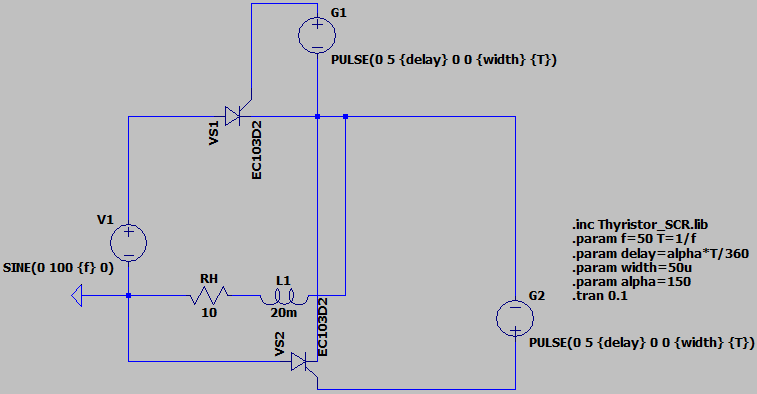
\includegraphics[scale=0.22]{scheme2.png}
        \captionsetup{skip=0pt}
        \caption{Подпись к изображению}
        \label{fig:scheme2}
    \end{figure}


    \begin{figure}[H]
        \centering
        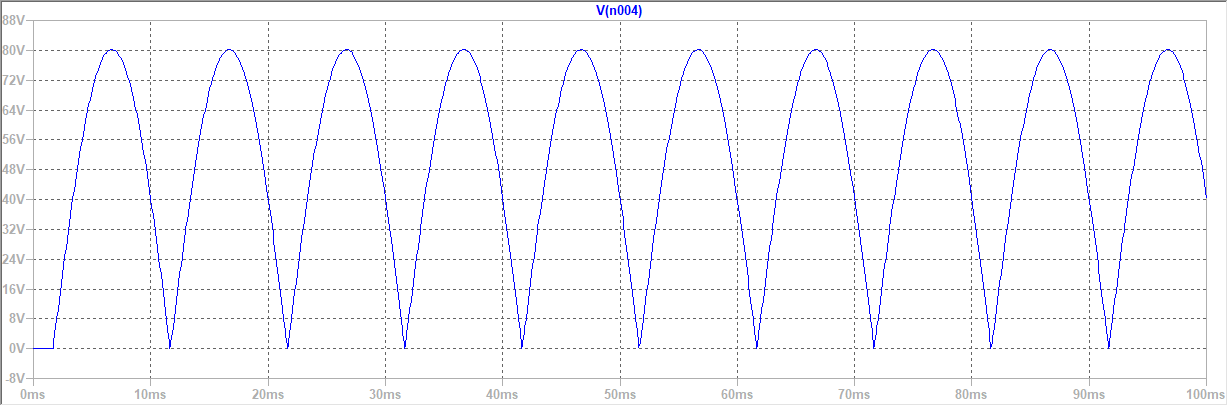
\includegraphics[scale=0.45]{a30_L20m.png}
        \captionsetup{skip=0pt}
        \caption{Подпись к изображению}
        \label{fig:a30_L20m}
    \end{figure}
    \begin{figure}[H]
        \centering
        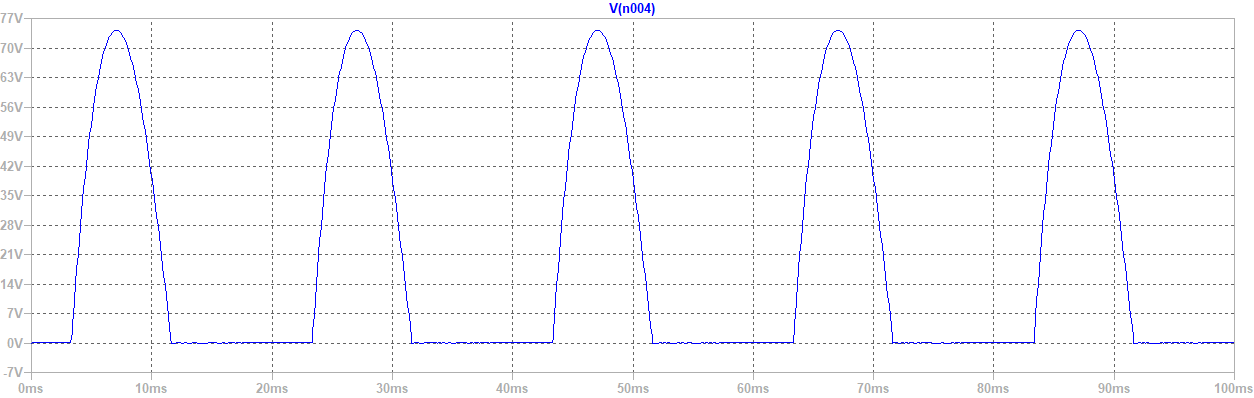
\includegraphics[scale=0.45]{a60_L20m.png}
        \captionsetup{skip=0pt}
        \caption{Подпись к изображению}
        \label{fig:a60_L20m}
    \end{figure}
    \begin{figure}[H]
        \centering
        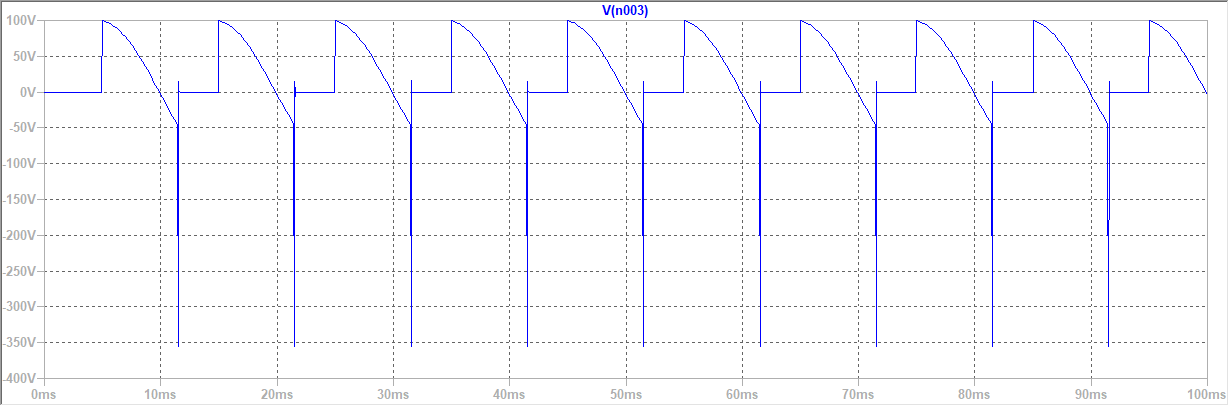
\includegraphics[scale=0.45]{a90_L20m.png}
        \captionsetup{skip=0pt}
        \caption{Подпись к изображению}
        \label{fig:a90_L20m}
    \end{figure}
    \begin{figure}[H]
        \centering
        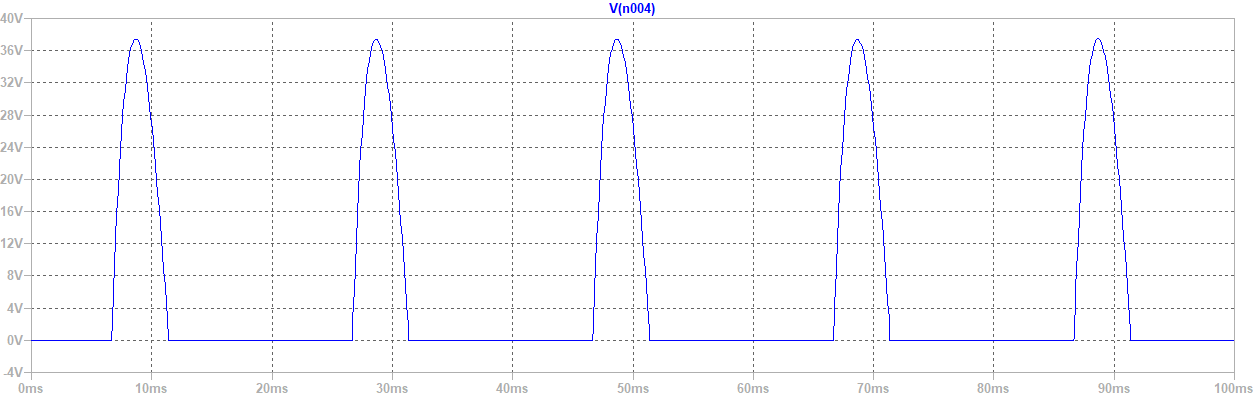
\includegraphics[scale=0.45]{a120_L20m.png}
        \captionsetup{skip=0pt}
        \caption{Подпись к изображению}
        \label{fig:a120_L20m}
    \end{figure}
    \begin{figure}[H]
        \centering
        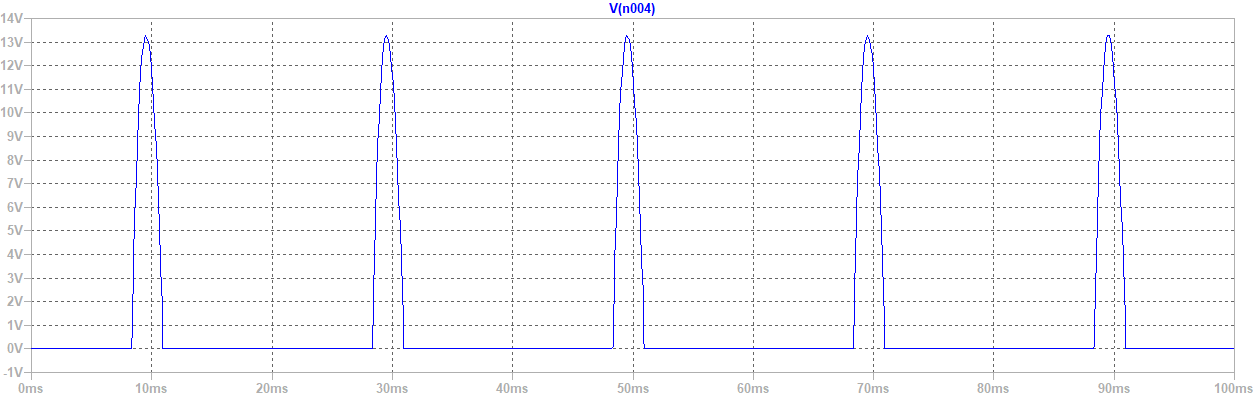
\includegraphics[scale=0.45]{a150_L20m.png}
        \captionsetup{skip=0pt}
        \caption{Подпись к изображению}
        \label{fig:a150_L20m}
    \end{figure}


    \begin{figure}[H]
        \centering
        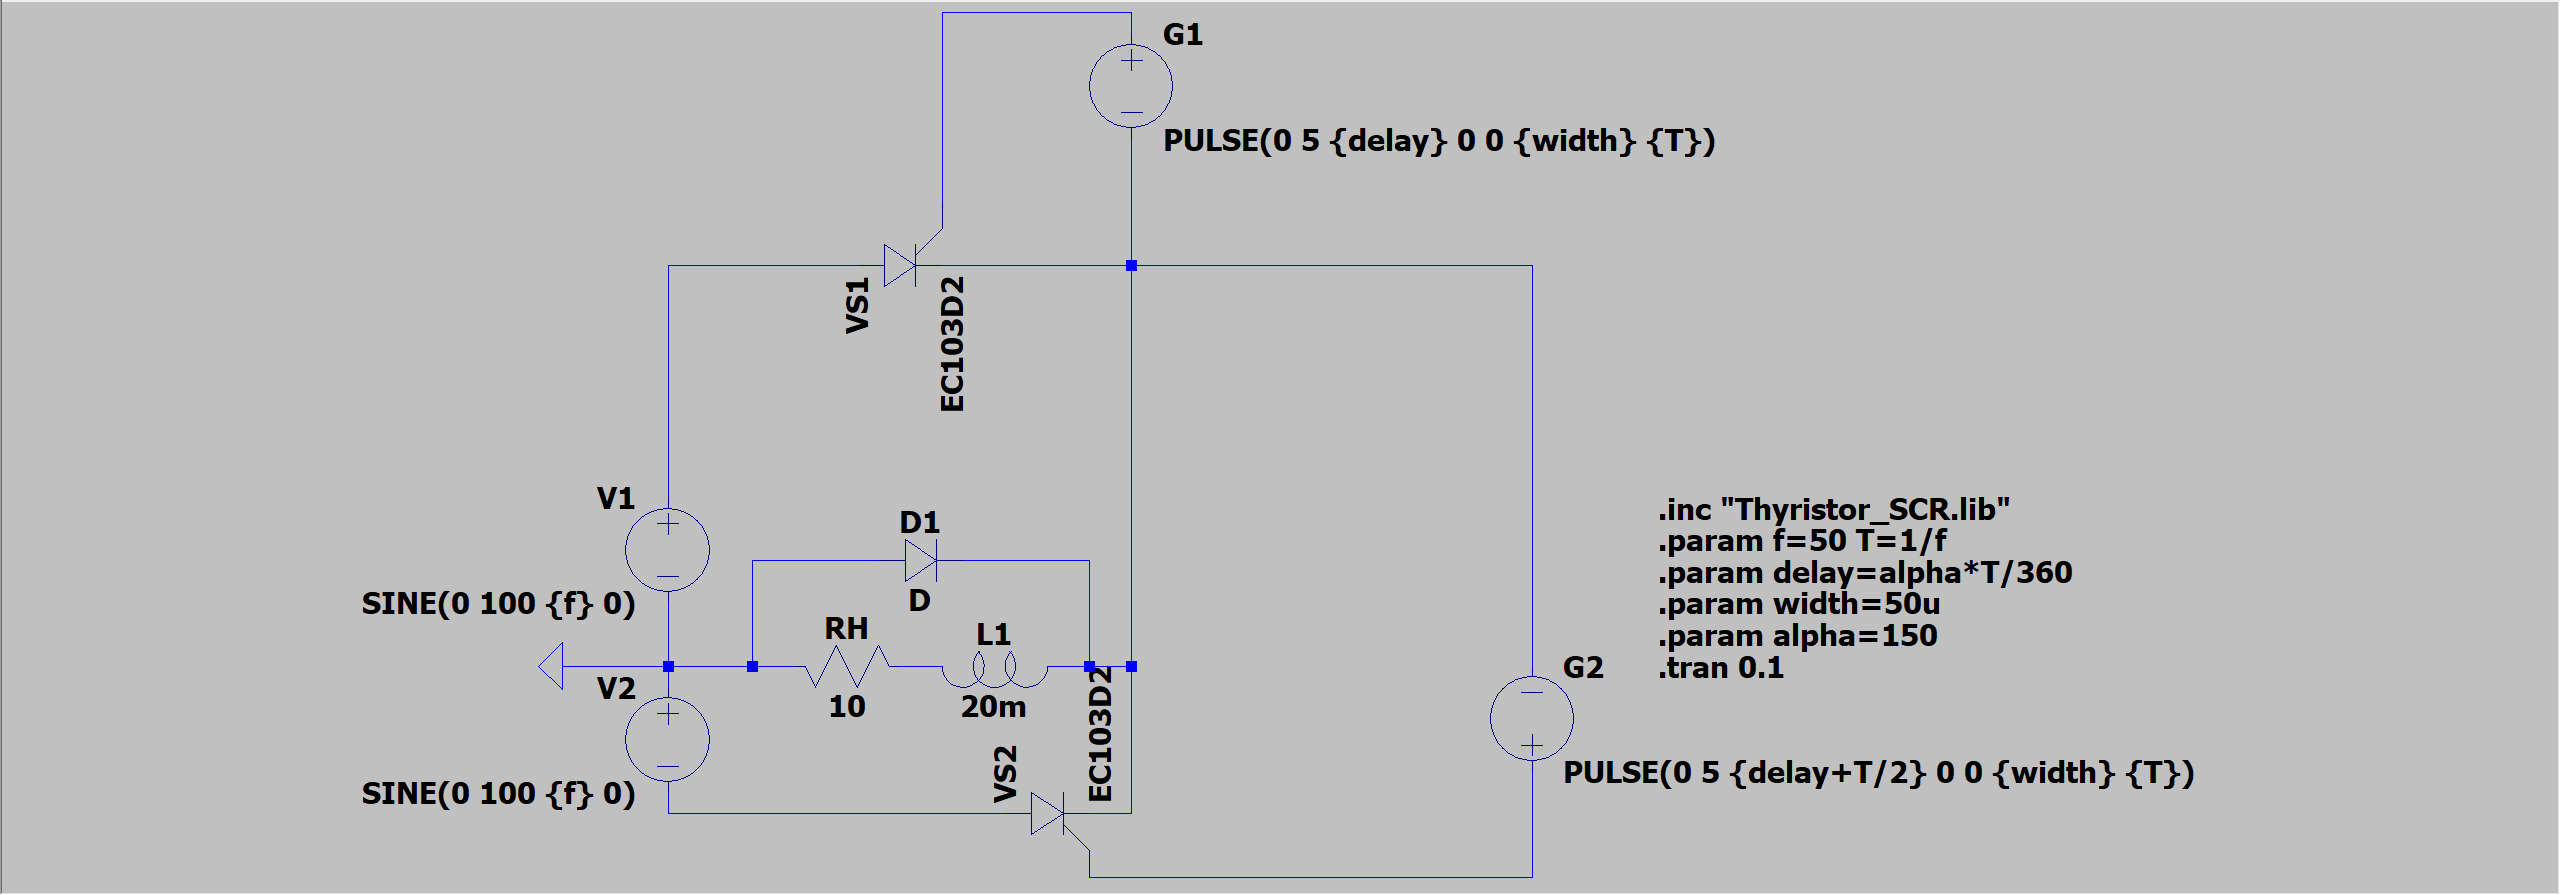
\includegraphics[scale=0.22]{scheme3.png}
        \captionsetup{skip=0pt}
        \caption{Подпись к изображению}
        \label{fig:scheme3}
    \end{figure}


    \begin{figure}[H]
        \centering
        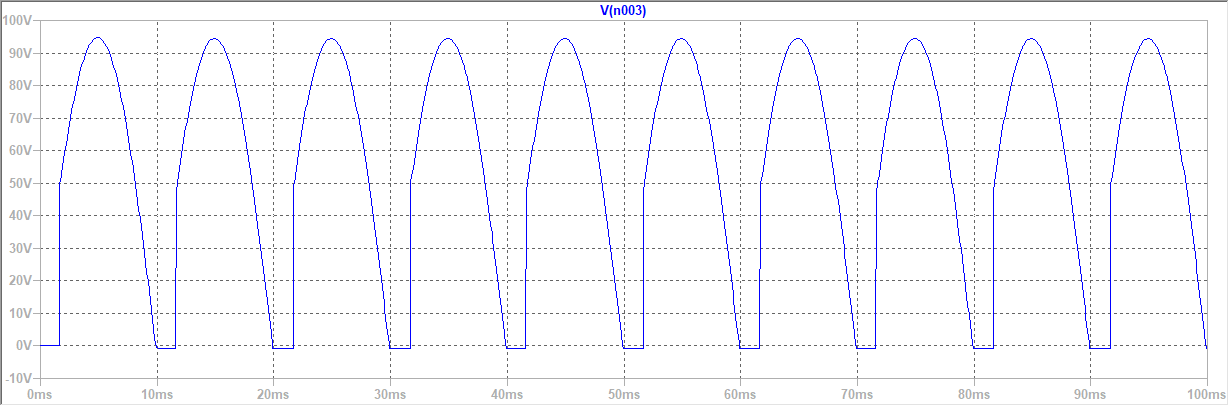
\includegraphics[scale=0.45]{a30_L20m_D.png}
        \captionsetup{skip=0pt}
        \caption{Подпись к изображению}
        \label{fig:a30_L20m_D}
    \end{figure}
    \begin{figure}[H]
        \centering
        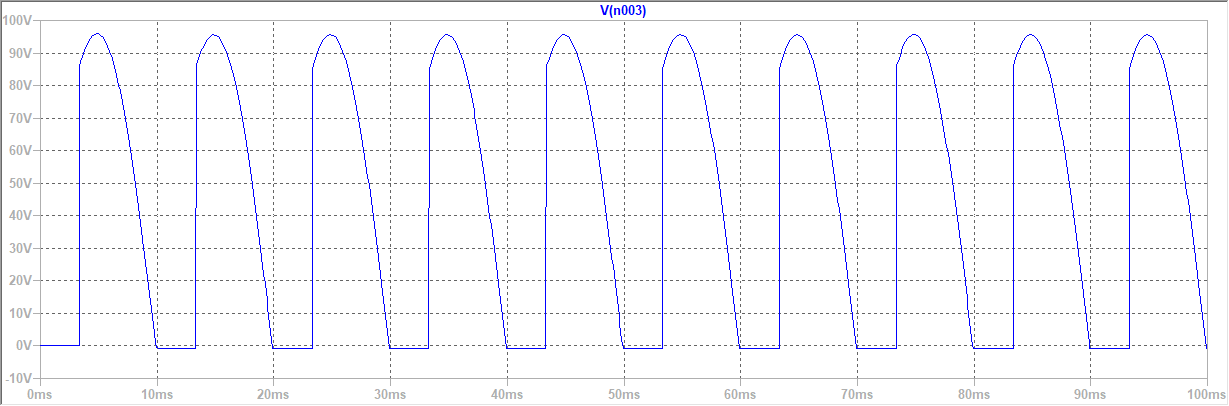
\includegraphics[scale=0.45]{a60_L20m_D.png}
        \captionsetup{skip=0pt}
        \caption{Подпись к изображению}
        \label{fig:a60_L20m_D}
    \end{figure}
    \begin{figure}[H]
        \centering
        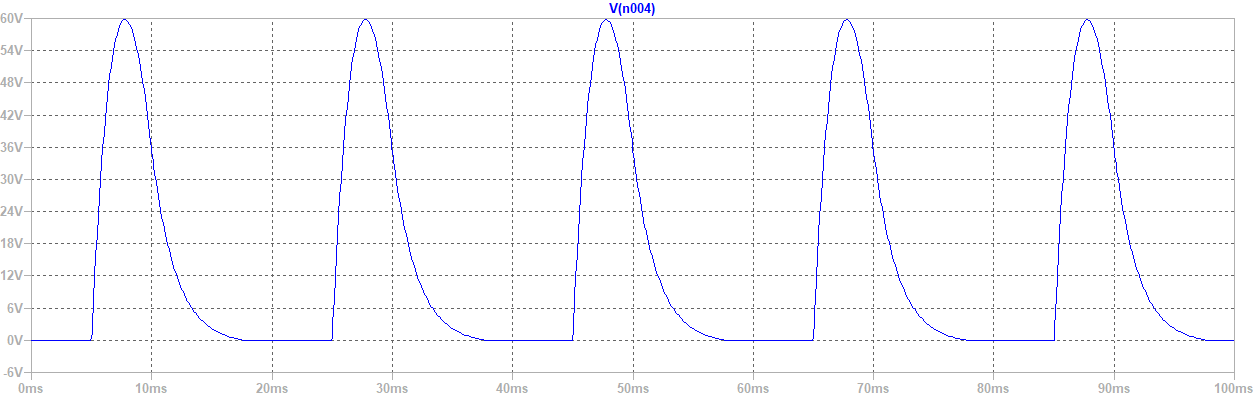
\includegraphics[scale=0.45]{a90_L20m_D.png}
        \captionsetup{skip=0pt}
        \caption{Подпись к изображению}
        \label{fig:a90_L20m_D}
    \end{figure}
    \begin{figure}[H]
        \centering
        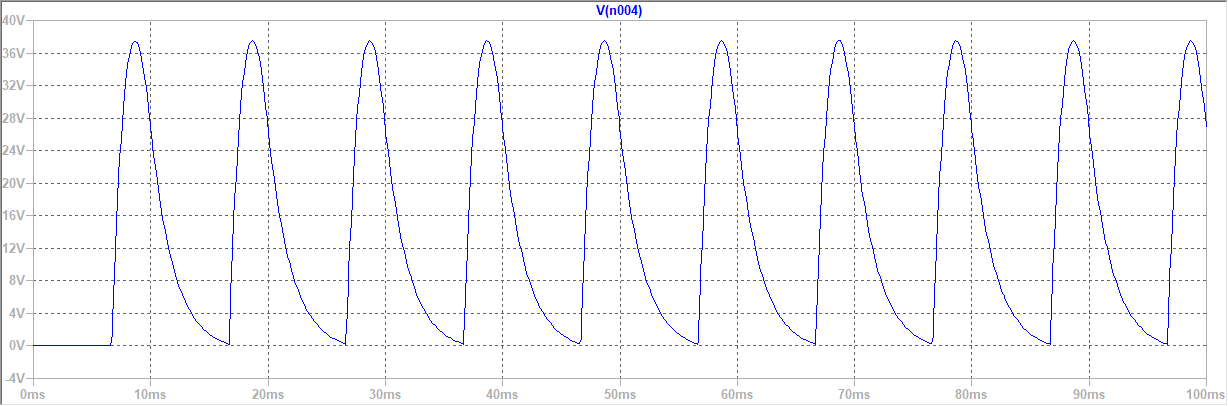
\includegraphics[scale=0.45]{a120_L20m_D.png}
        \captionsetup{skip=0pt}
        \caption{Подпись к изображению}
        \label{fig:a120_L20m_D}
    \end{figure}
    \begin{figure}[H]
        \centering
        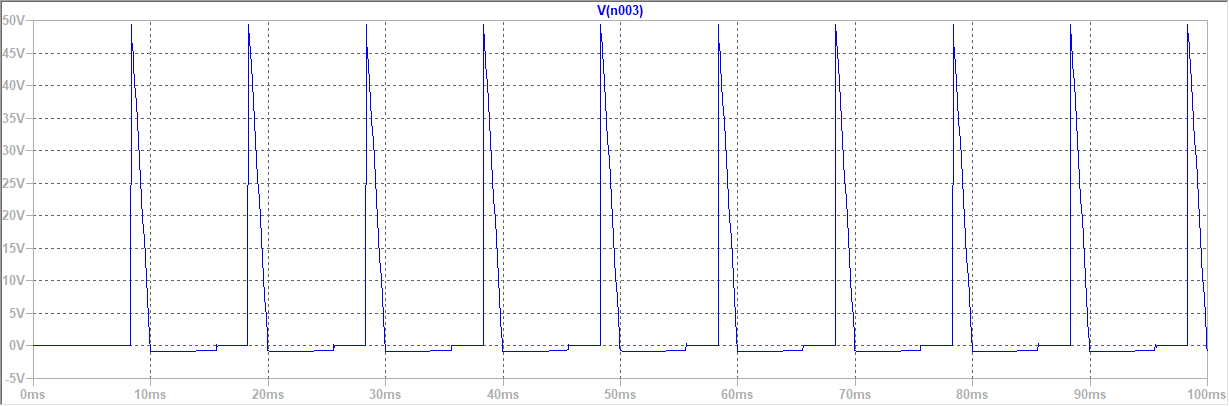
\includegraphics[scale=0.45]{a150_L20m_D.png}
        \captionsetup{skip=0pt}
        \caption{Подпись к изображению}
        \label{fig:a150_L20m_D}
    \end{figure}


    \section{Задание 2}
    \begin{figure}[H]
        \centering
        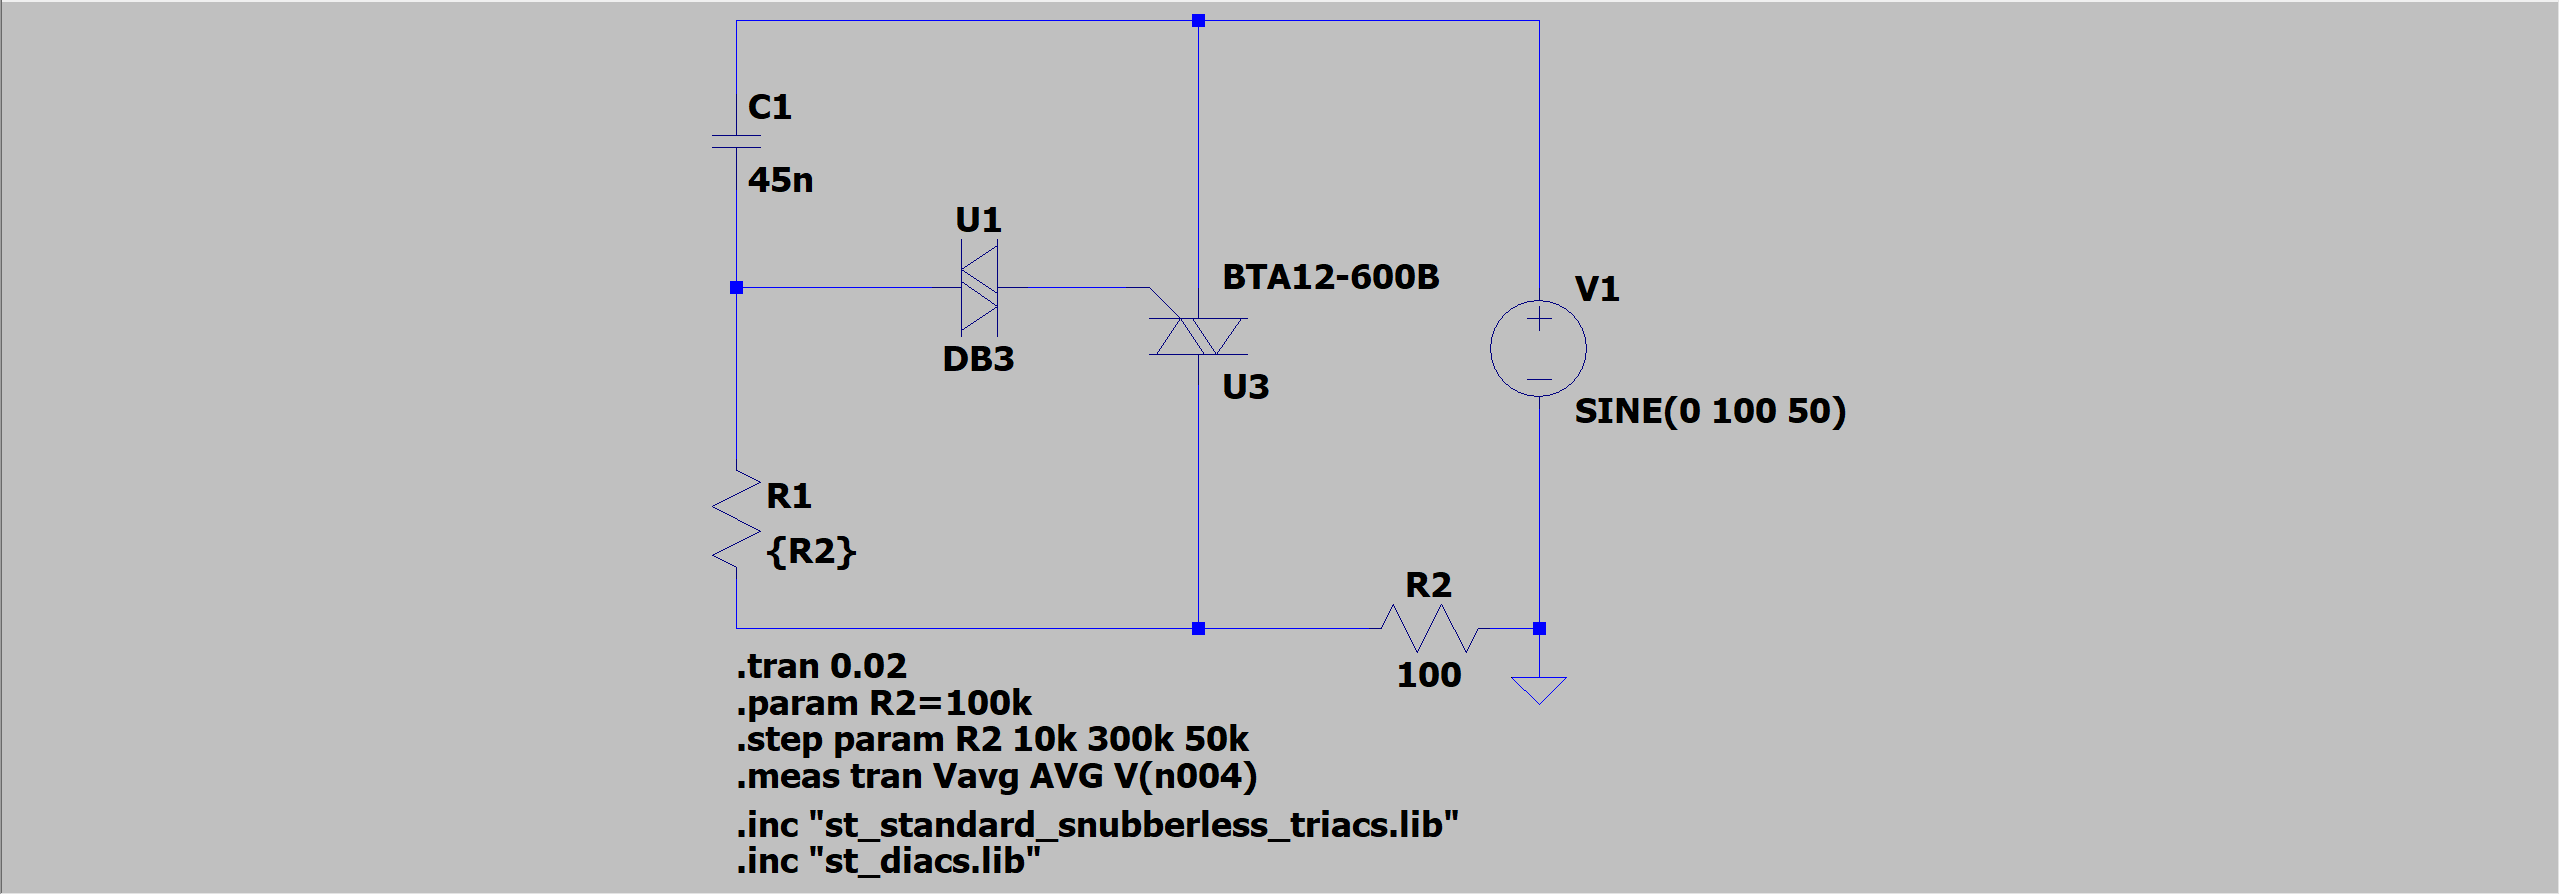
\includegraphics[scale=0.3]{scheme4.png}
        \captionsetup{skip=0pt}
        \caption{Подпись к изображению}
        \label{fig:scheme4}
    \end{figure}


    \subsection{Вых}
    \begin{center}
        \begin{tabular}{ | m{4em} | m{1.5cm}| m{1.5cm} | m{1.5cm} | m{1.5cm} | m{1.5cm} | m{1.5cm} | m{1.5cm} | } 
        \hline
        $R,k$& 10 & 60 & 110 &160 &210 &260 &300 \\ 
        \hline
        $U_{out}$& 0.0263 & 0.3374 & 1.2721 &2.731 &4.6158 &7.8872 &3.2499\\ 
        \hline
    \end{tabular}
    \end{center}


    \begin{figure}[H]
        \centering
        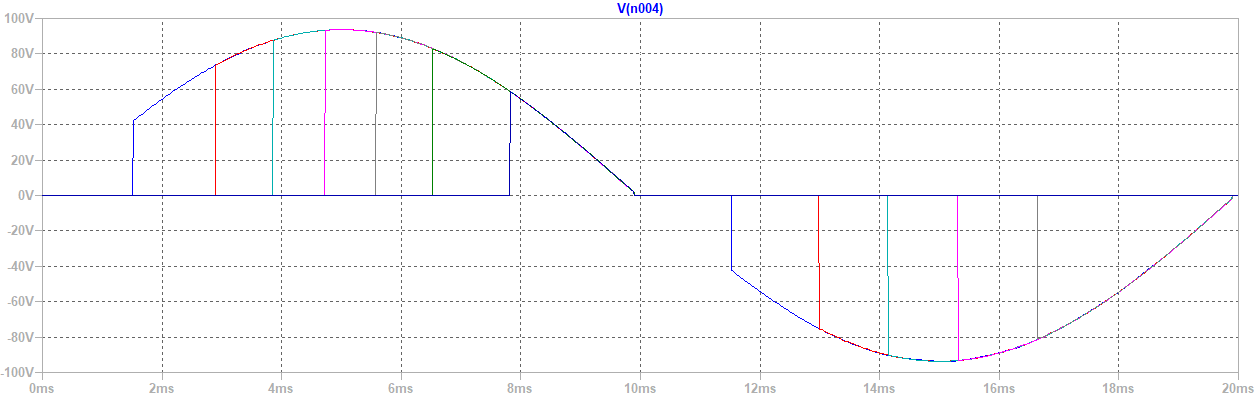
\includegraphics[scale=0.45]{R2-all.png}
        \captionsetup{skip=0pt}
        \caption{Подпись к изображению}
        \label{fig:R2-all}
    \end{figure}


    \begin{figure}[H]
        \centering
        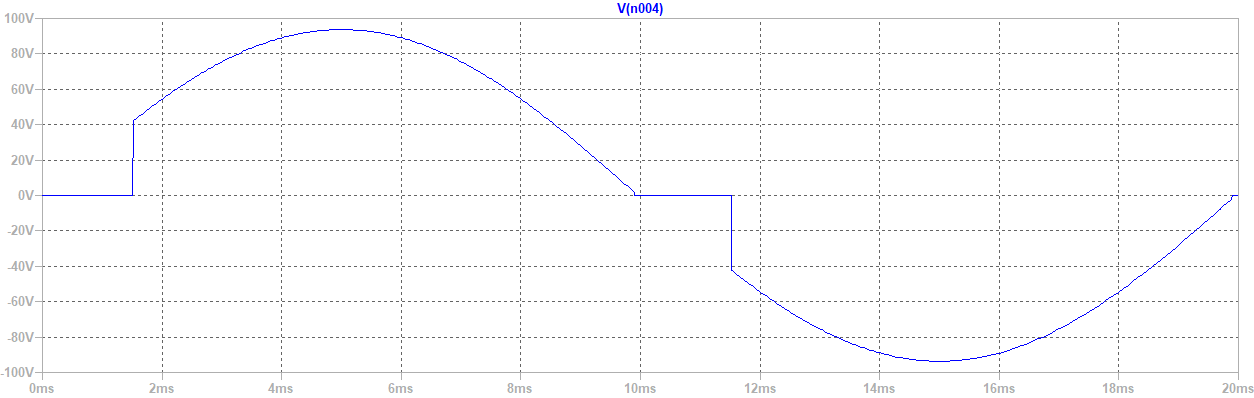
\includegraphics[scale=0.45]{R2-10k.png}
        \captionsetup{skip=0pt}
        \caption{Подпись к изображению}
        \label{fig:R2-10k}
    \end{figure}
    \begin{figure}[H]
        \centering
        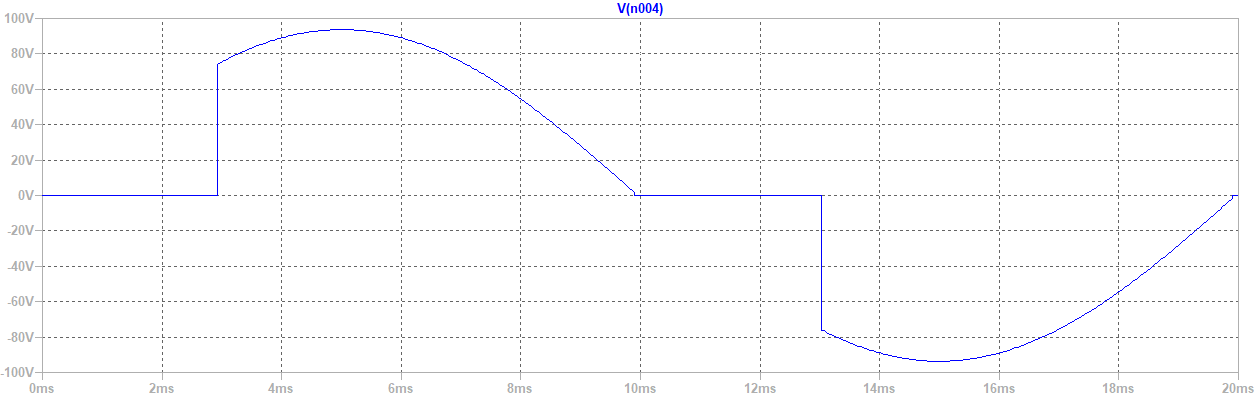
\includegraphics[scale=0.45]{R2-60k.png}
        \captionsetup{skip=0pt}
        \caption{Подпись к изображению}
        \label{fig:R2-60k}
    \end{figure}
    \begin{figure}[H]
        \centering
        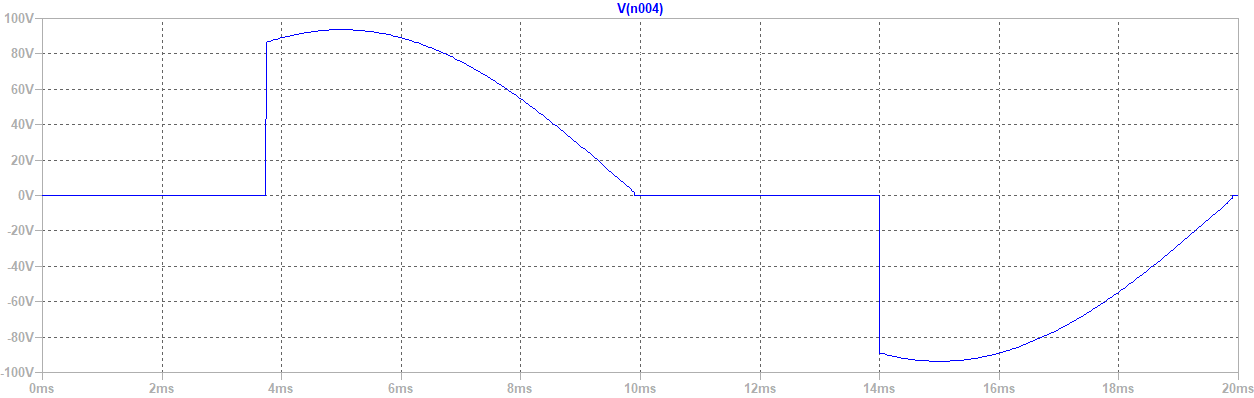
\includegraphics[scale=0.45]{R2-100k.png}
        \captionsetup{skip=0pt}
        \caption{Подпись к изображению}
        \label{fig:R2-100k}
    \end{figure}
    \begin{figure}[H]
        \centering
        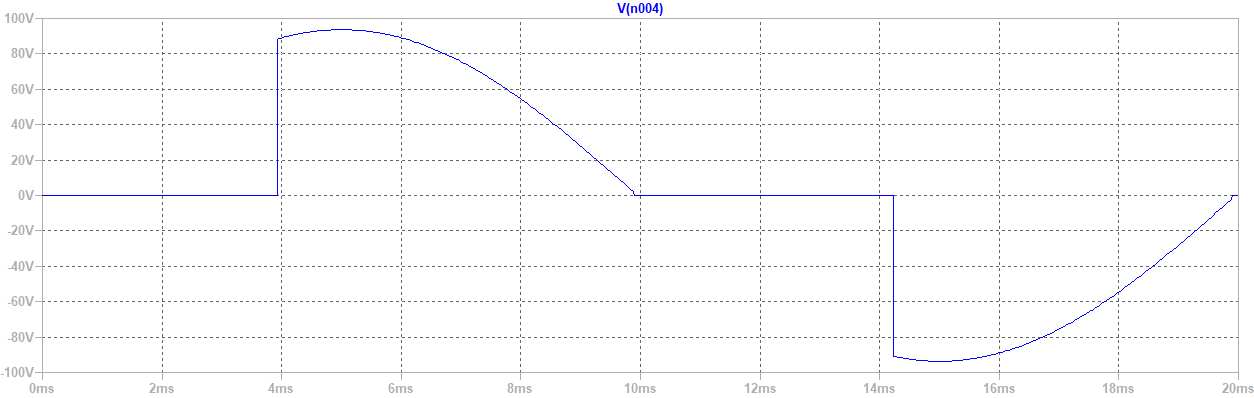
\includegraphics[scale=0.45]{R2-110k.png}
        \captionsetup{skip=0pt}
        \caption{Подпись к изображению}
        \label{fig:R2-110k}
    \end{figure}
    \begin{figure}[H]
        \centering
        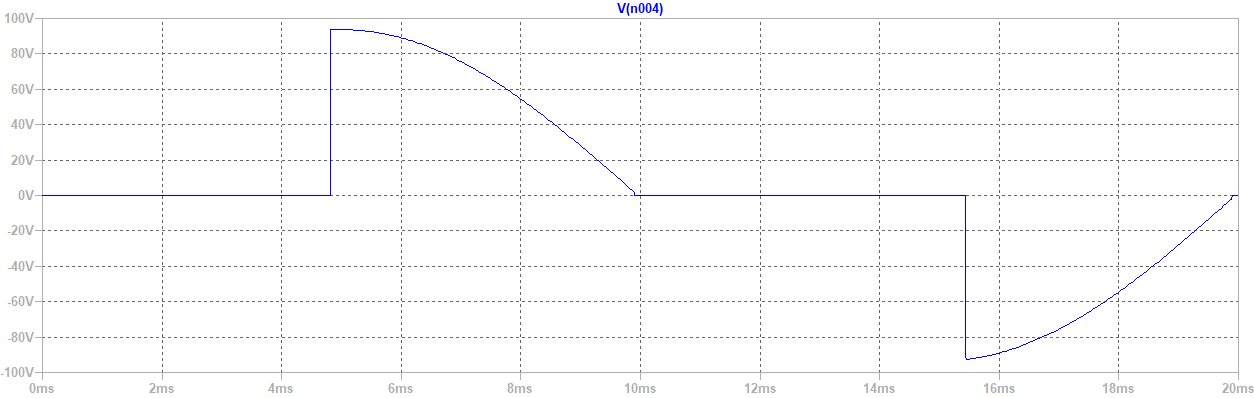
\includegraphics[scale=0.45]{R2-160k.png}
        \captionsetup{skip=0pt}
        \caption{Подпись к изображению}
        \label{fig:R2-160k}
    \end{figure}
    \begin{figure}[H]
        \centering
        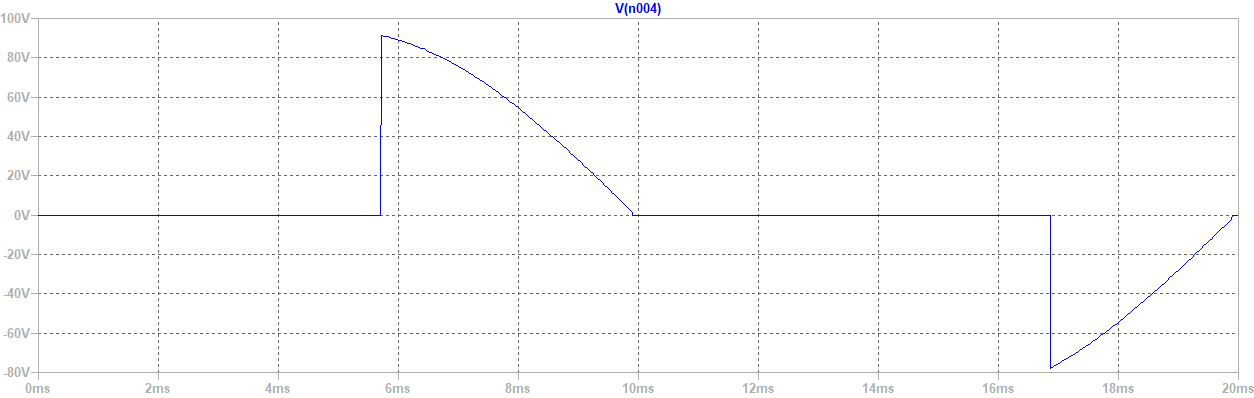
\includegraphics[scale=0.45]{R2-210k.png}
        \captionsetup{skip=0pt}
        \caption{Подпись к изображению}
        \label{fig:R2-210k}
    \end{figure}
    \begin{figure}[H]
        \centering
        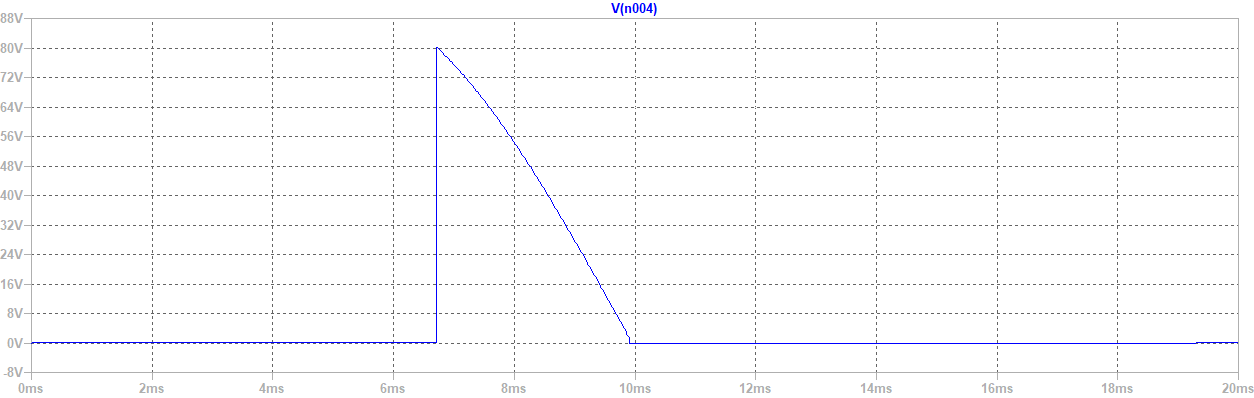
\includegraphics[scale=0.45]{R2-260k.png}
        \captionsetup{skip=0pt}
        \caption{Подпись к изображению}
        \label{fig:R2-260k}
    \end{figure}
    \begin{figure}[H]
        \centering
        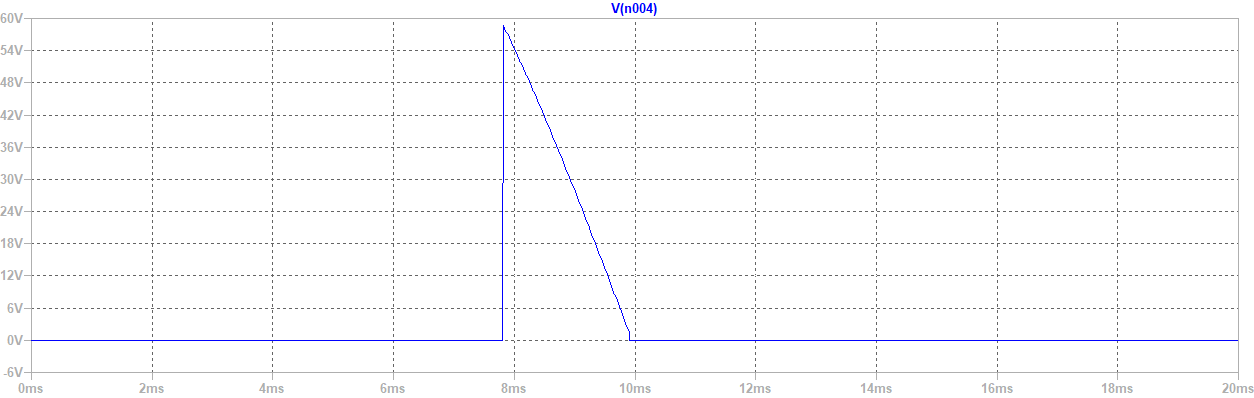
\includegraphics[scale=0.45]{R2-300k.png}
        \captionsetup{skip=0pt}
        \caption{Подпись к изображению}
        \label{fig:R2-300k}
    \end{figure}


    \begin{figure}[H]
        \centering
        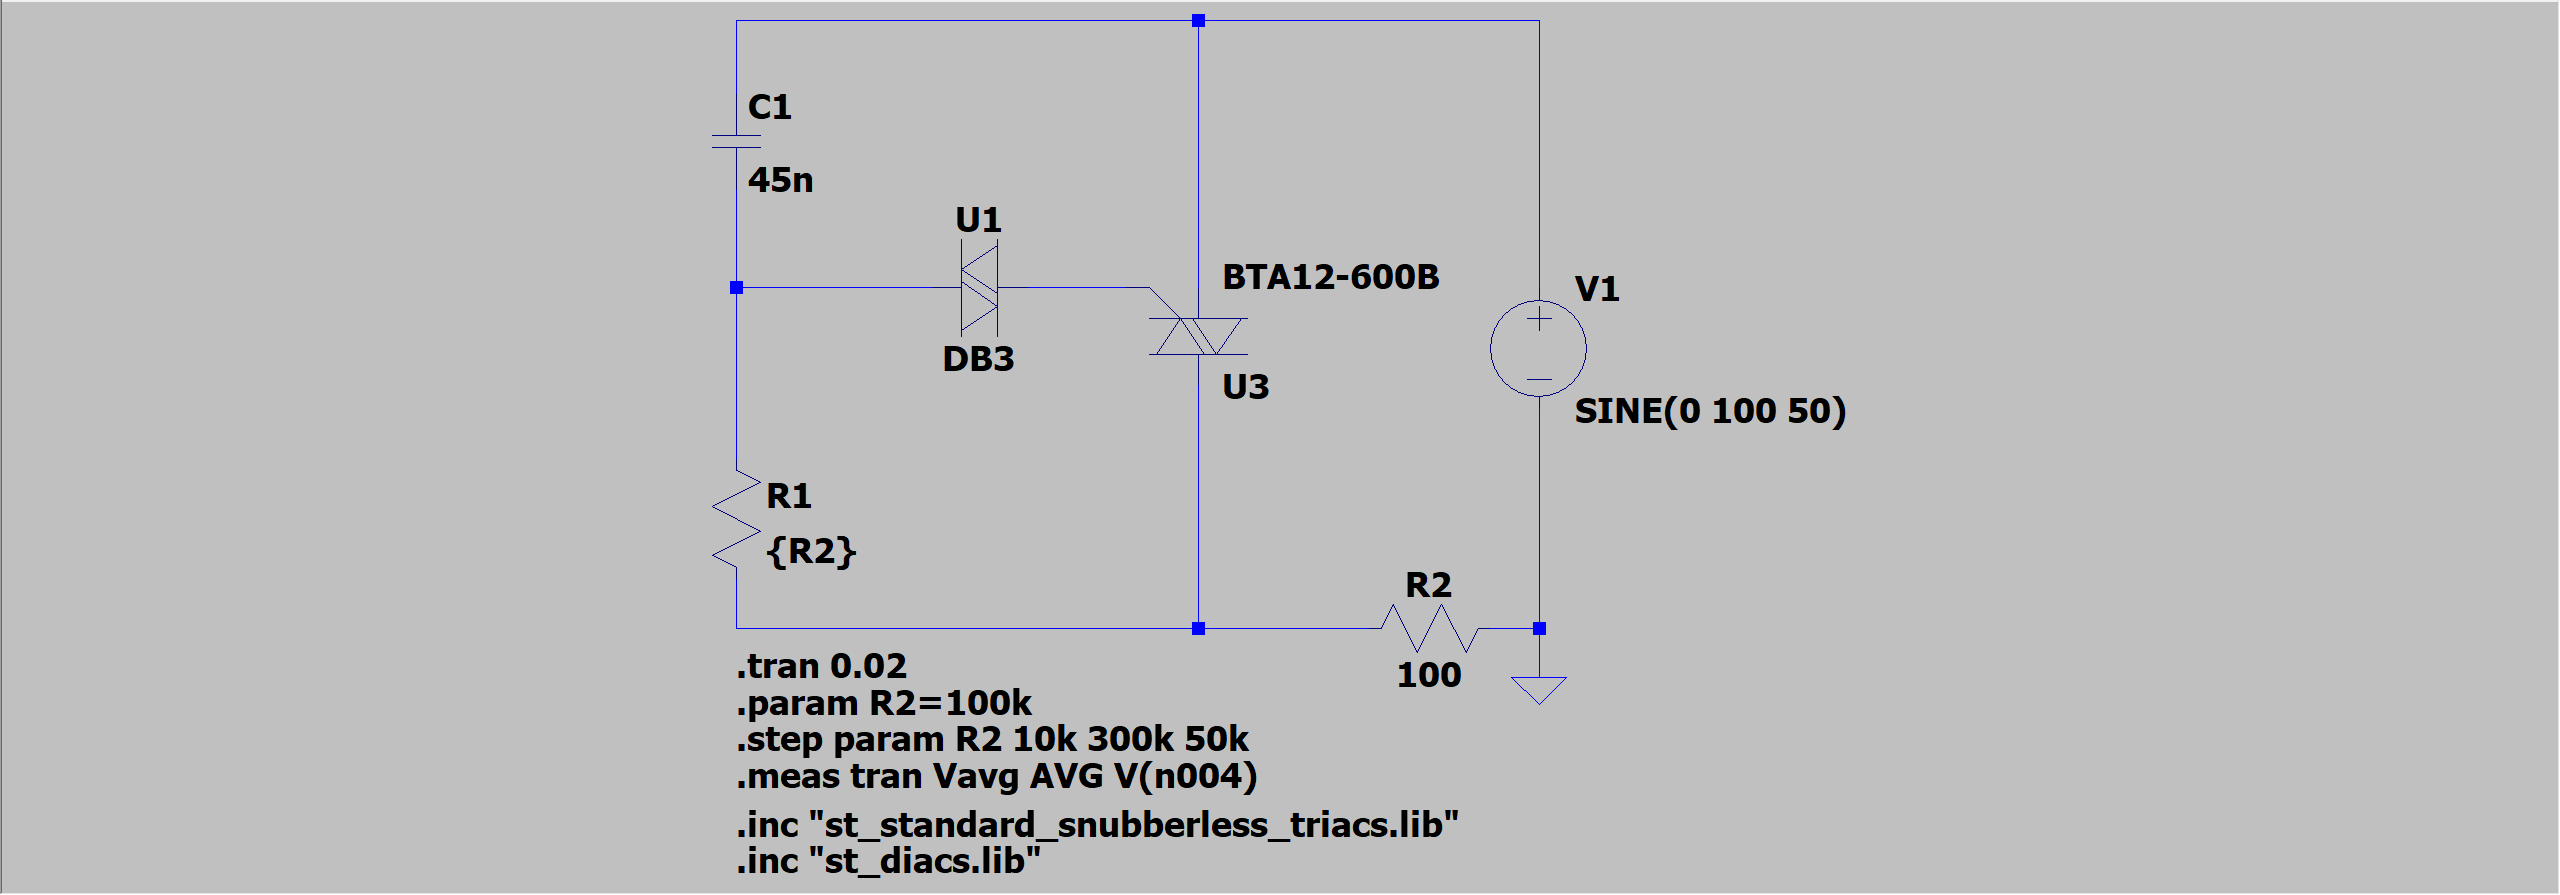
\includegraphics[scale=0.3]{scheme5.png}
        \captionsetup{skip=0pt}
        \caption{Подпись к изображению}
        \label{fig:scheme5}
    \end{figure}


    \begin{figure}[H]
        \centering
        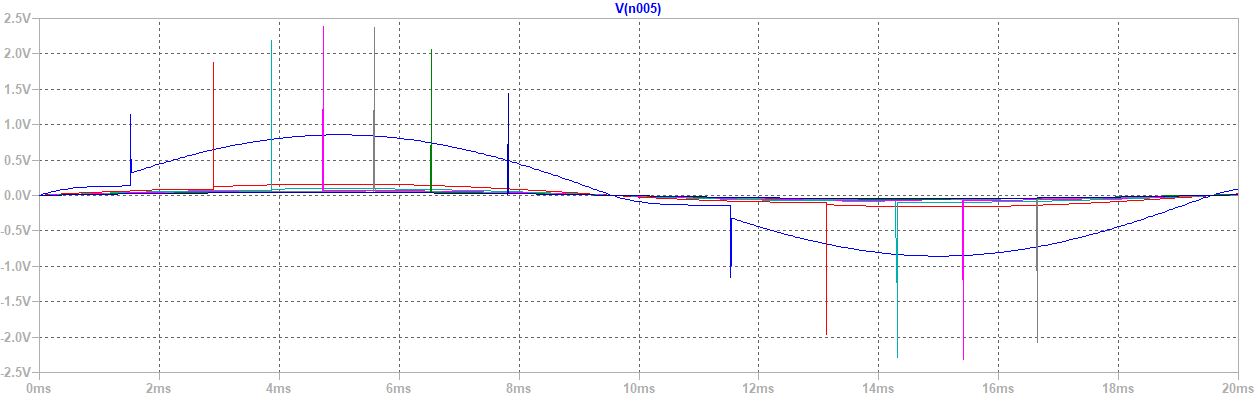
\includegraphics[scale=0.45]{R2-all_L20m.png}
        \captionsetup{skip=0pt}
        \caption{Подпись к изображению}
        \label{fig:R2-all_L20m}
    \end{figure}


    \begin{figure}[H]
        \centering
        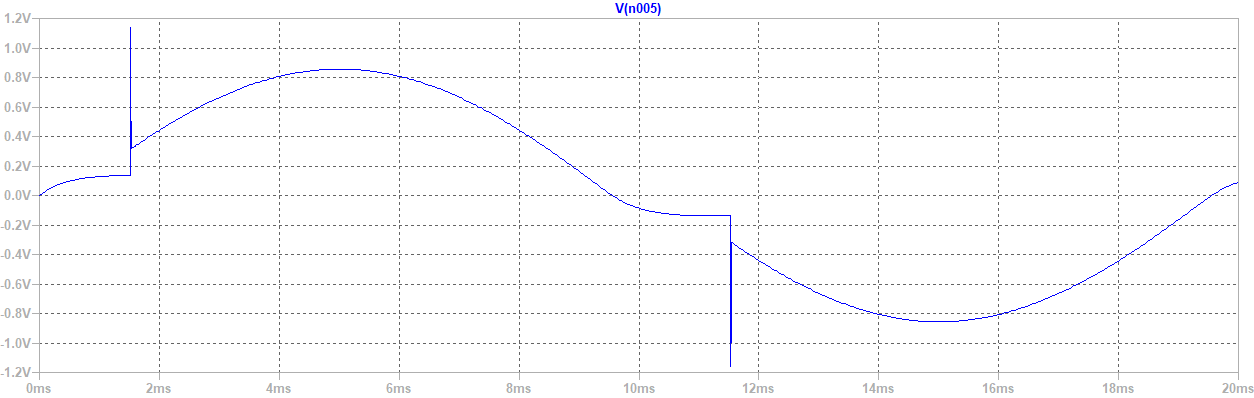
\includegraphics[scale=0.45]{R2-10k_L20m.png}
        \captionsetup{skip=0pt}
        \caption{Подпись к изображению}
        \label{fig:R2-10k_L20m}
    \end{figure}
    \begin{figure}[H]
        \centering
        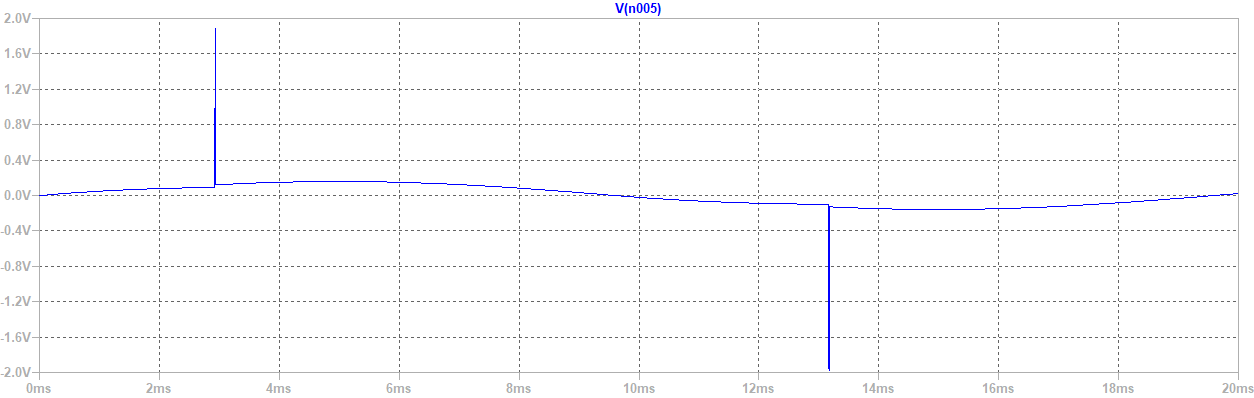
\includegraphics[scale=0.45]{R2-60k_L20m.png}
        \captionsetup{skip=0pt}
        \caption{Подпись к изображению}
        \label{fig:R2-60k_L20m}
    \end{figure}
    \begin{figure}[H]
        \centering
        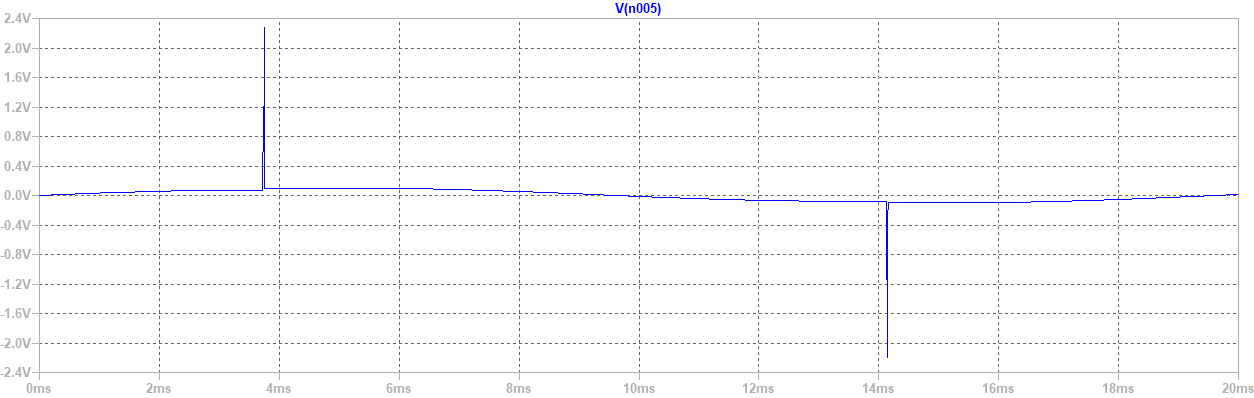
\includegraphics[scale=0.45]{R2-100k_L20m.png}
        \captionsetup{skip=0pt}
        \caption{Подпись к изображению}
        \label{fig:R2-100k_L20m}
    \end{figure}
    \begin{figure}[H]
        \centering
        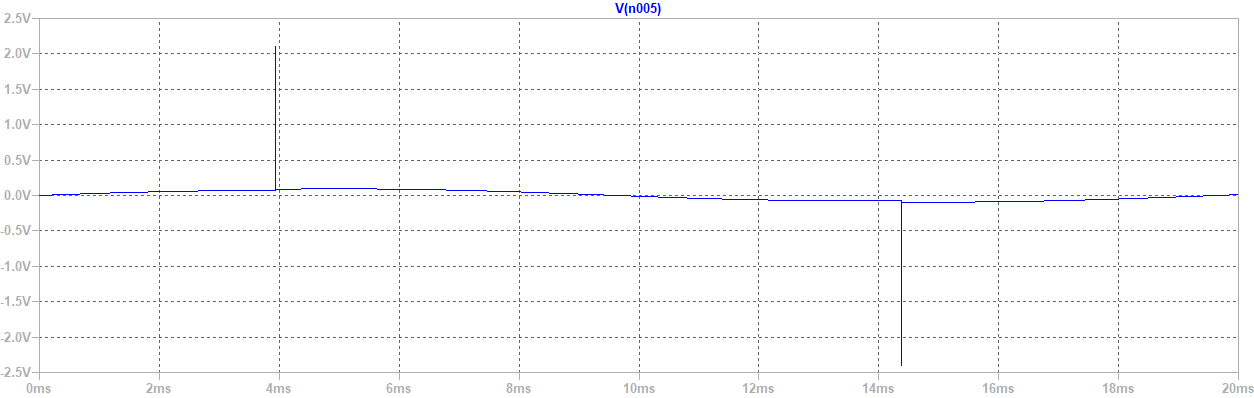
\includegraphics[scale=0.45]{R2-110k_L20m.png}
        \captionsetup{skip=0pt}
        \caption{Подпись к изображению}
        \label{fig:R2-110k_L20m}
    \end{figure}
    \begin{figure}[H]
        \centering
        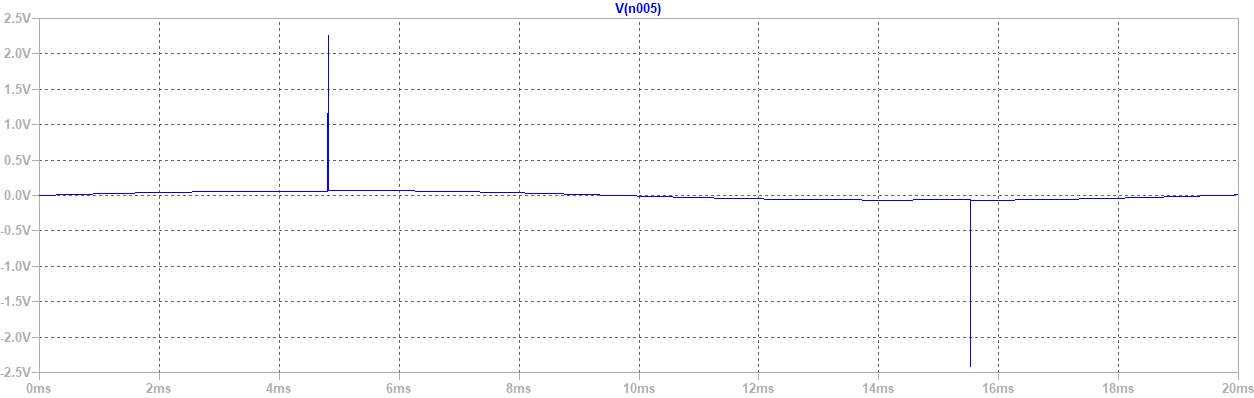
\includegraphics[scale=0.45]{R2-160k_L20m.png}
        \captionsetup{skip=0pt}
        \caption{Подпись к изображению}
        \label{fig:R2-160k_L20m}
    \end{figure}
    \begin{figure}[H]
        \centering
        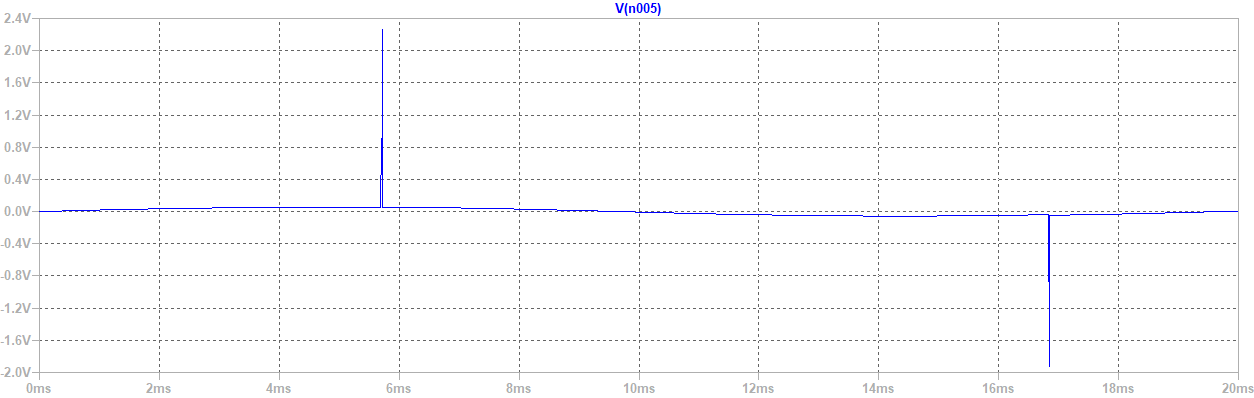
\includegraphics[scale=0.45]{R2-210k_L20m.png}
        \captionsetup{skip=0pt}
        \caption{Подпись к изображению}
        \label{fig:R2-210k_L20m}
    \end{figure}
    \begin{figure}[H]
        \centering
        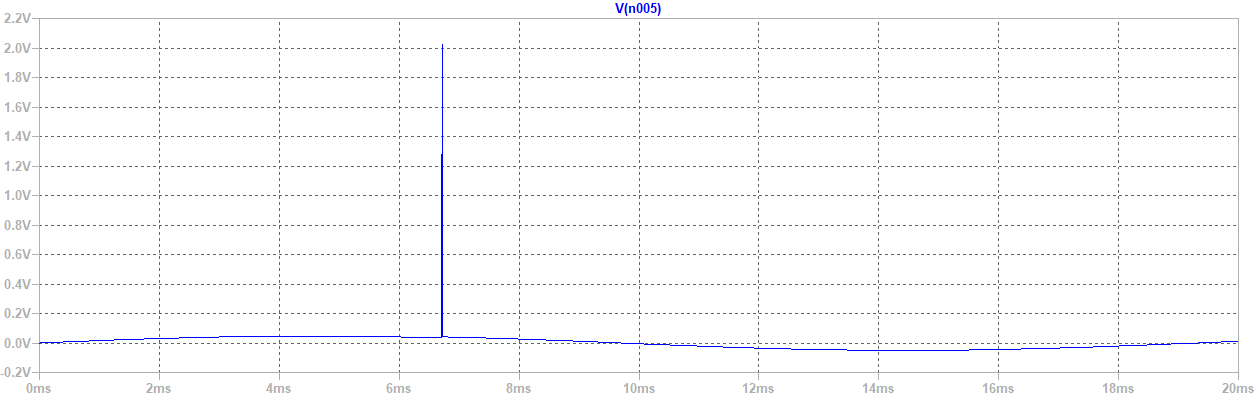
\includegraphics[scale=0.45]{R2-260k_L20m.png}
        \captionsetup{skip=0pt}
        \caption{Подпись к изображению}
        \label{fig:R2-260k_L20m}
    \end{figure}
    \begin{figure}[H]
        \centering
        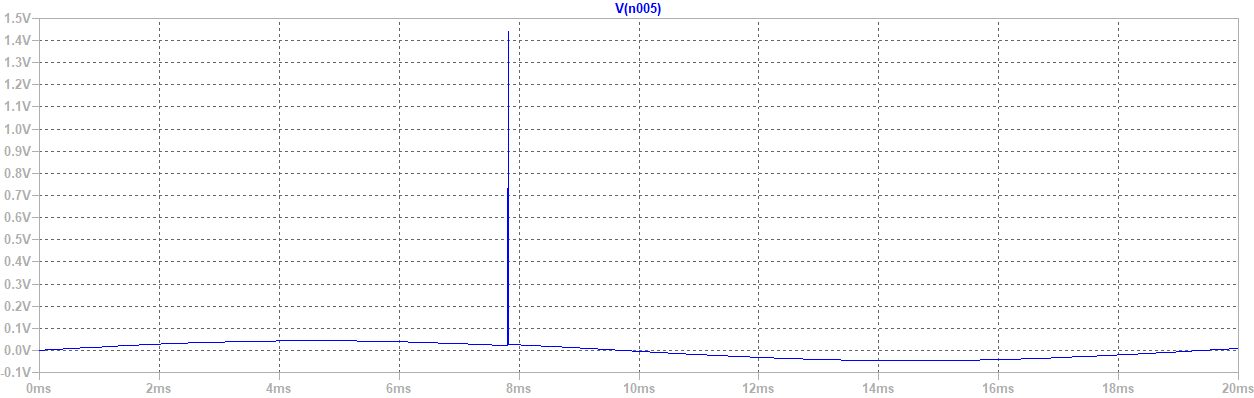
\includegraphics[scale=0.45]{R2-300k_L20m.png}
        \captionsetup{skip=0pt}
        \caption{Подпись к изображению}
        \label{fig:R2-300k_L20m}
    \end{figure}


    \begin{figure}[H]
        \centering
        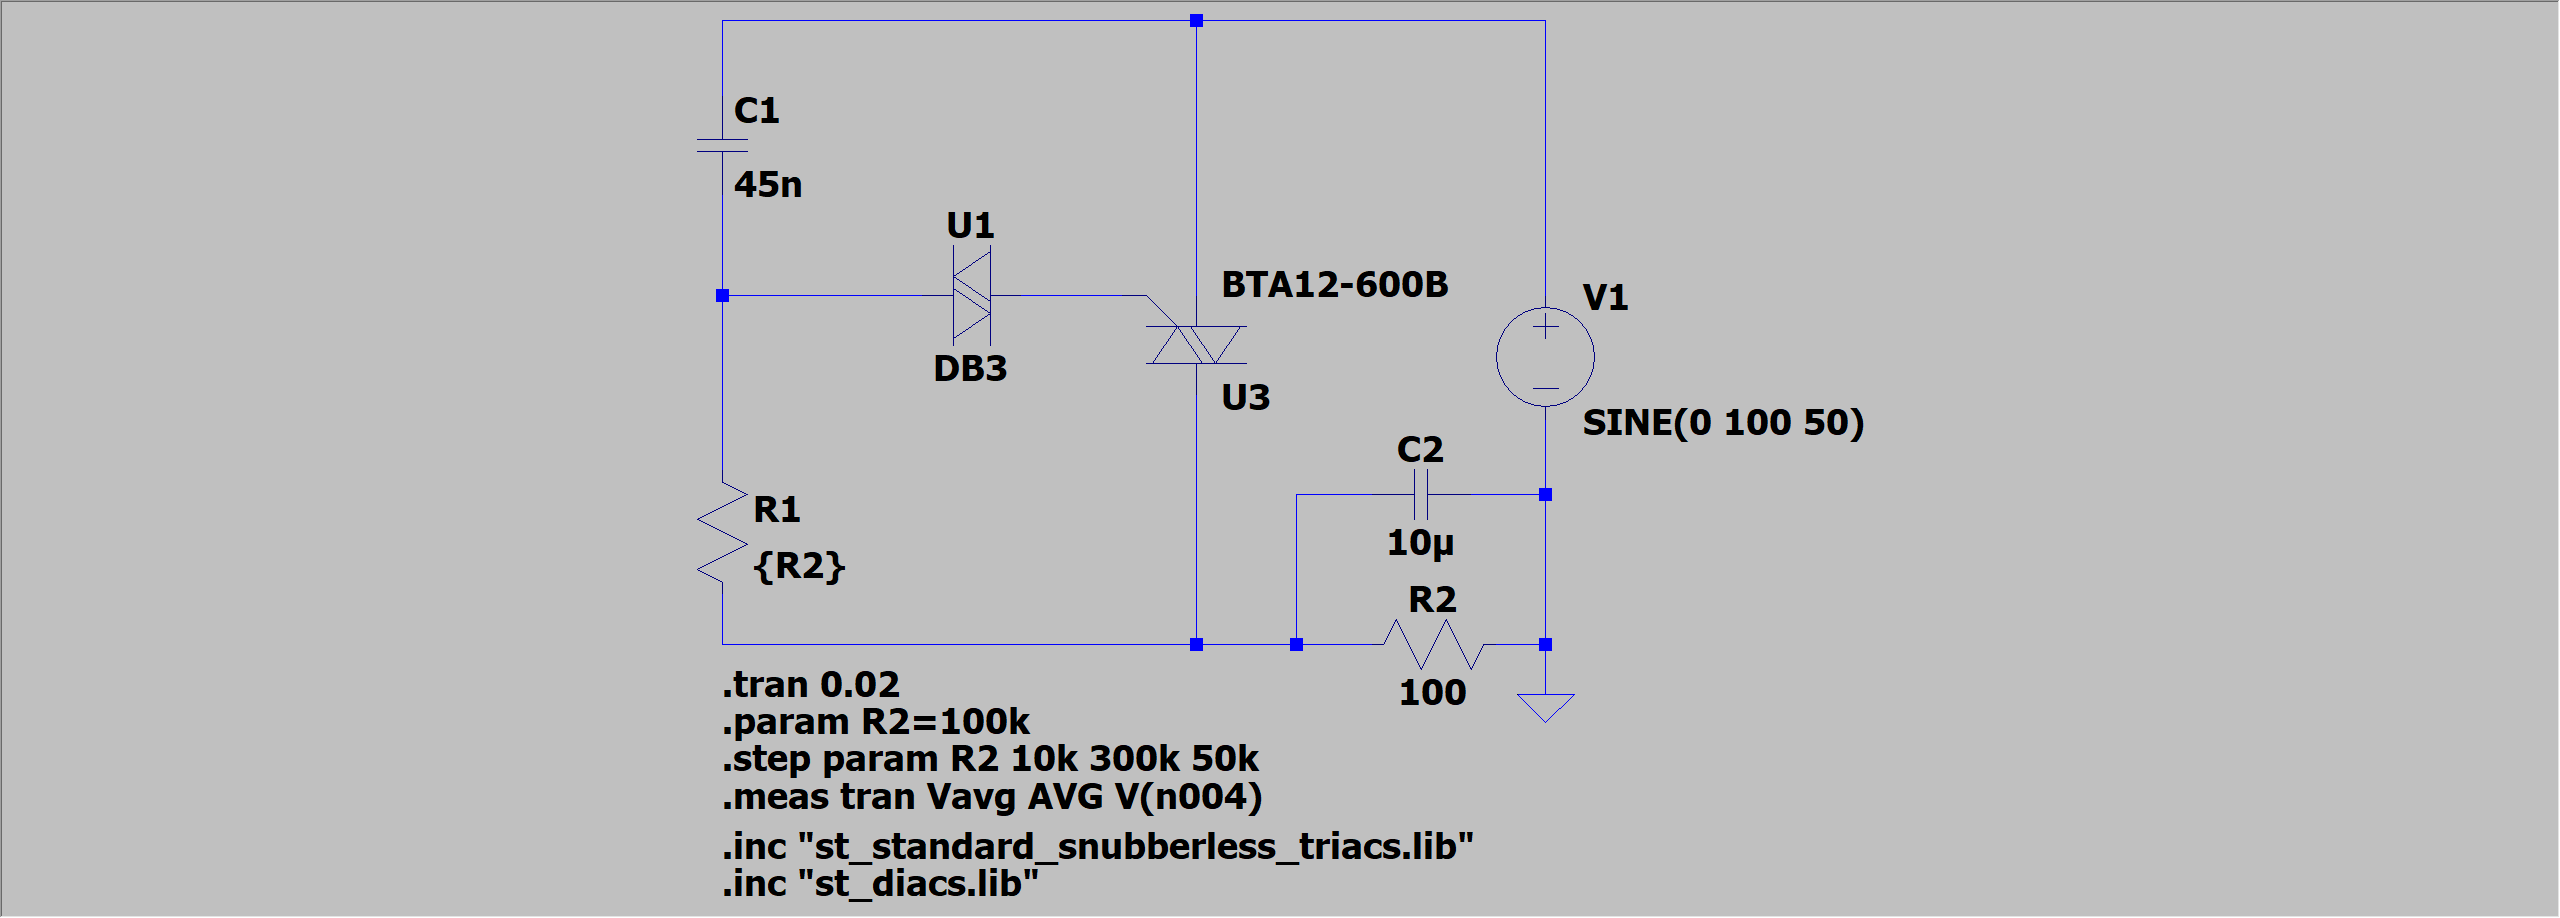
\includegraphics[scale=0.3]{scheme6.png}
        \captionsetup{skip=0pt}
        \caption{Подпись к изображению}
        \label{fig:scheme6}
    \end{figure}


    \begin{figure}[H]
        \centering
        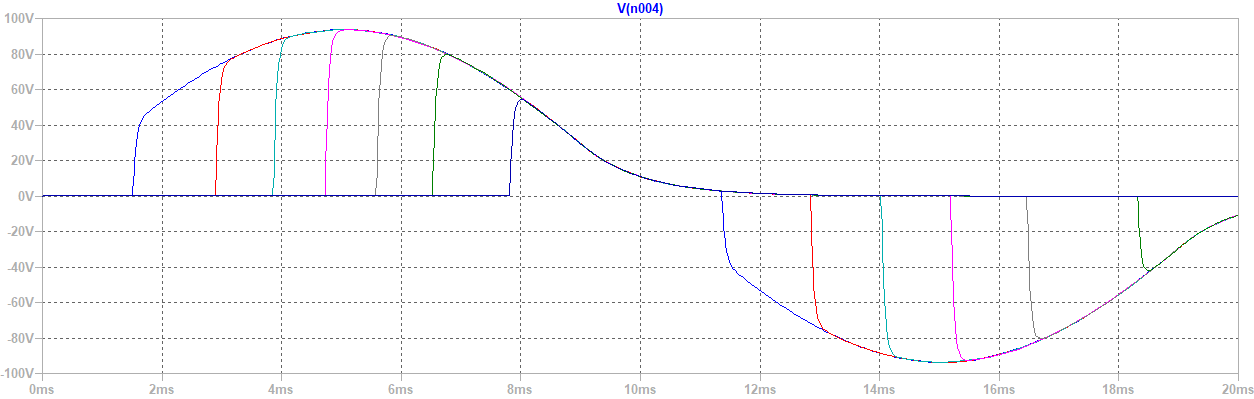
\includegraphics[scale=0.45]{R2-all_C10u.png}
        \captionsetup{skip=0pt}
        \caption{Подпись к изображению}
        \label{fig:R2-all_C10u}
    \end{figure}


    \begin{figure}[H]
        \centering
        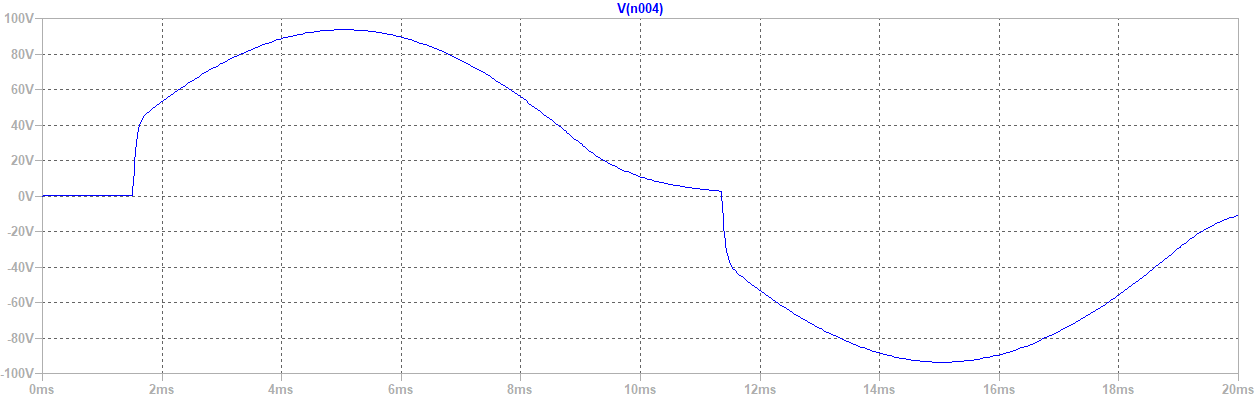
\includegraphics[scale=0.45]{R2-10k_C10u.png}
        \captionsetup{skip=0pt}
        \caption{Подпись к изображению}
        \label{fig:R2-10k_C10u}
    \end{figure}
    \begin{figure}[H]
        \centering
        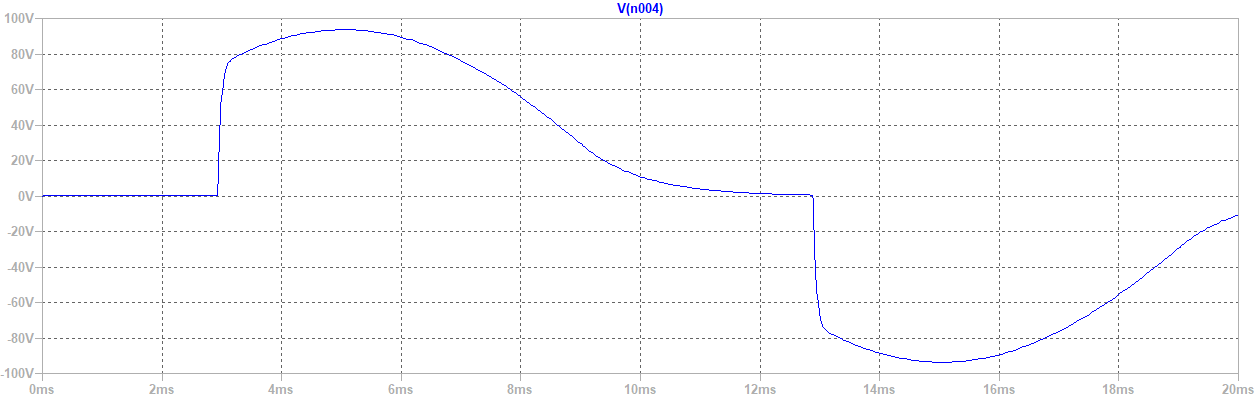
\includegraphics[scale=0.45]{R2-60k_C10u.png}
        \captionsetup{skip=0pt}
        \caption{Подпись к изображению}
        \label{fig:R2-60k_C10u}
    \end{figure}
    \begin{figure}[H]
        \centering
        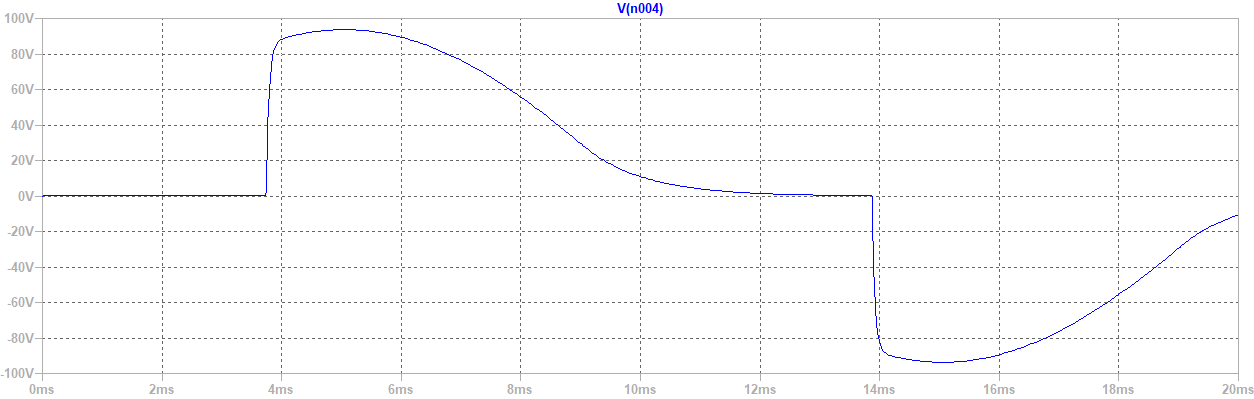
\includegraphics[scale=0.45]{R2-100k_C10u.png}
        \captionsetup{skip=0pt}
        \caption{Подпись к изображению}
        \label{fig:R2-100k_C10u}
    \end{figure}
    \begin{figure}[H]
        \centering
        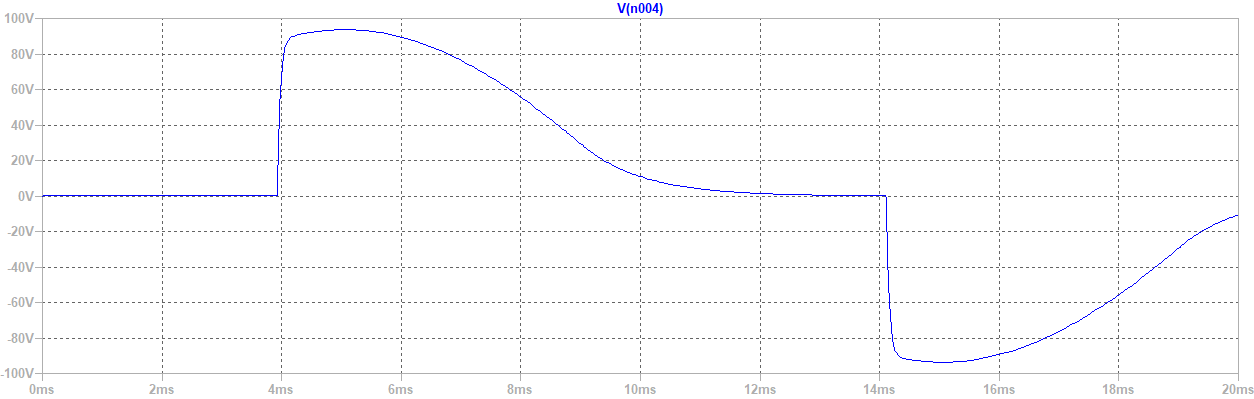
\includegraphics[scale=0.45]{R2-110k_C10u.png}
        \captionsetup{skip=0pt}
        \caption{Подпись к изображению}
        \label{fig:R2-110k_C10u}
    \end{figure}
    \begin{figure}[H]
        \centering
        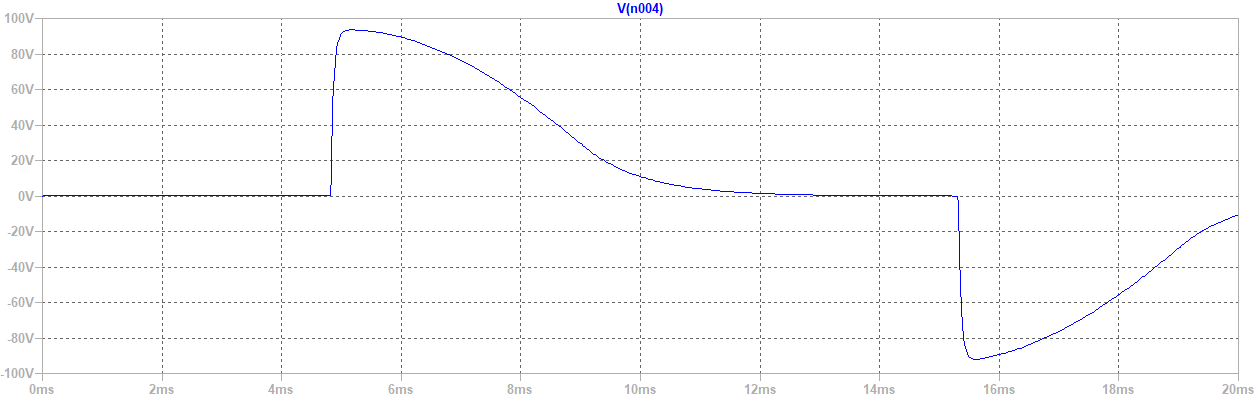
\includegraphics[scale=0.45]{R2-160k_C10u.png}
        \captionsetup{skip=0pt}
        \caption{Подпись к изображению}
        \label{fig:R2-160k_C10u}
    \end{figure}
    \begin{figure}[H]
        \centering
        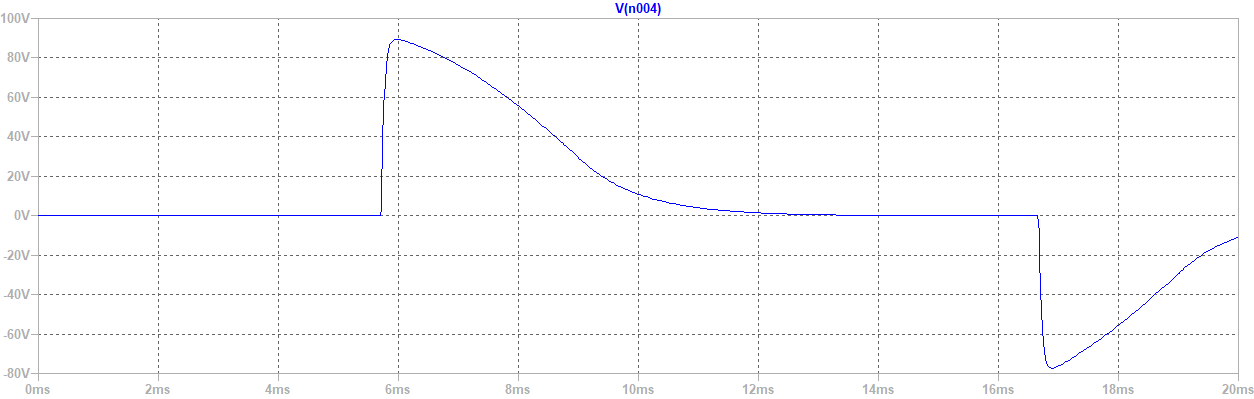
\includegraphics[scale=0.45]{R2-210k_C10u.png}
        \captionsetup{skip=0pt}
        \caption{Подпись к изображению}
        \label{fig:R2-210k_C10u}
    \end{figure}
    \begin{figure}[H]
        \centering
        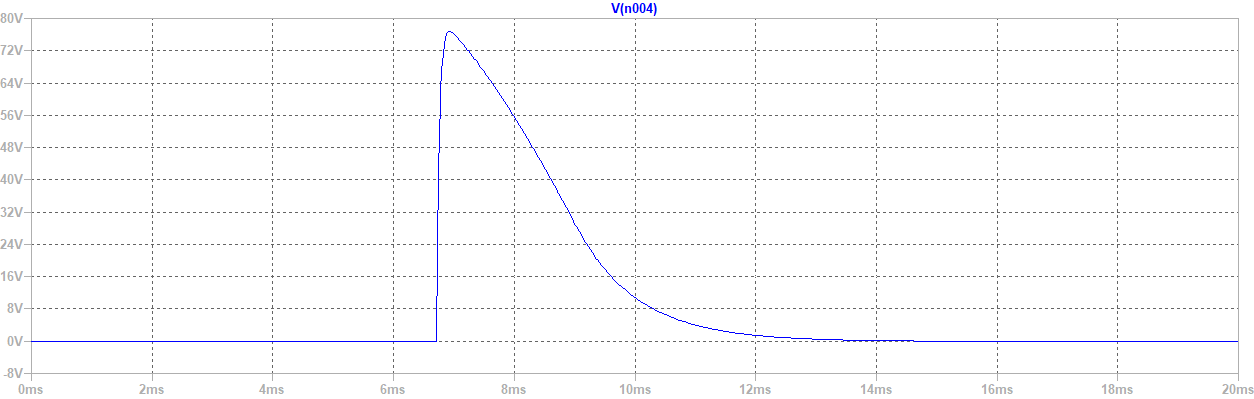
\includegraphics[scale=0.45]{R2-260k_C10u.png}
        \captionsetup{skip=0pt}
        \caption{Подпись к изображению}
        \label{fig:R2-260k_C10u}
    \end{figure}
    \begin{figure}[H]
        \centering
        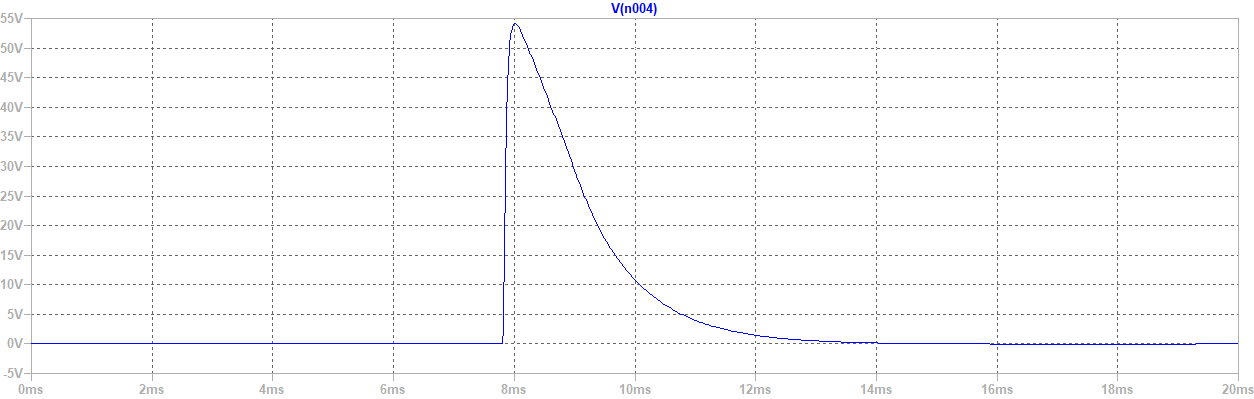
\includegraphics[scale=0.45]{R2-300k_C10u.png}
        \captionsetup{skip=0pt}
        \caption{Подпись к изображению}
        \label{fig:R2-300k_C10u}
    \end{figure}


    \section{Вывод}
    ...


\end{document}